% !TeX root = ../documento.tex
\chapter{Metodologia Específica: Controle Digital Para um Sistema de Freio ACC}
\label{cap:controle}

O Controle de Cruzeiro Adaptativo (ACC) constitui uma tecnologia relevante nos veículos modernos, especialmente em contextos de direção assistida e autônoma. Sua principal função é ajustar automaticamente a velocidade do veículo para manter uma distância segura em relação ao veículo à frente, promovendo conforto, segurança e eficiência no trânsito.


Embora existam diversas abordagens teóricas para o desenvolvimento de sistemas ACC, a aplicação prática ainda apresenta desafios consideráveis. Muitos trabalhos concentram-se em simulações e modelagens teóricas, enquanto a implementação em hardware embarcado permanece menos explorada na literatura.

Neste estudo, busca-se contribuir para essa lacuna ao propor e validar um sistema de controle digital para o freio veicular com base em ACC, utilizando o microcontrolador automotivo AURIX TC375. O desenvolvimento inclui uma placa de controle dedicada, modelagem do sistema em espaço de estados e a aplicação de técnicas de controle digital. A validação é realizada por meio de simulações no MATLAB/Simulink e testes práticos em ambiente controlado, visando analisar a viabilidade da solução em condições representativas.

O sistema proposto foi desenvolvido para: 
\begin{itemize} 
    \item Investigar a capacidade de manter a distância segura em relação ao veículo à frente; 
    \item Avaliar o controle da pressão de frenagem de forma precisa e responsiva; 
    \item Explorar a implementação em hardware real, com sensores e atuadores automotivos. 
\end{itemize}

A Figura~\ref{fig:Acc_tabela_de_distancias} apresenta uma tabela que relaciona a distância de relativa $d$, a desaceleração $a$, e a velocidade relativa máxima $v_{\text{rel}}$ que pode ser compensada com segurança, conforme a equação:

\begin{equation}
v_{\text{rel}} = -\sqrt{2d \cdot a}
\end{equation}

Essa expressão, derivada sob a hipótese de desaceleração uniforme e trajetória retilínea, fornece um limite operacional para o ACC em situações de aproximação rápida. Dessa forma, a tabela serve como referência para definir valores seguros de desaceleração a serem empregadas na geração do sinal $a_{\text{des}}$ utilizado nas simulações subsequentes.

\begin{figure}[htbp]
    \centering
    \caption{Tabela de Distâncias para o Sistema ACC}
    \label{fig:Acc_tabela_de_distancias}
    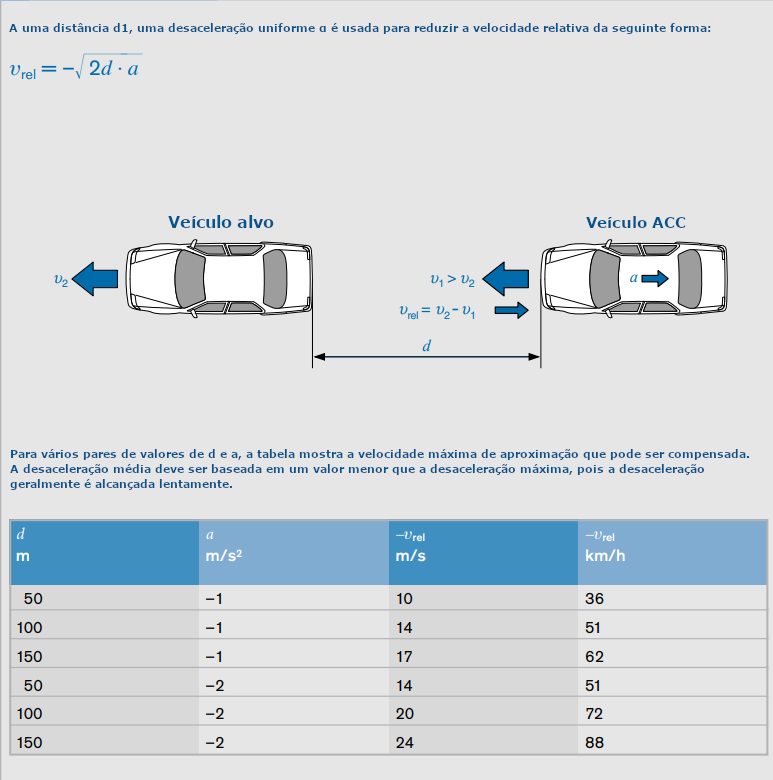
\includegraphics[width=0.8\textwidth]{figuras/Acc_tabela_de_distancias.png}
    \fonte{ O Autor, adaptado de \cite{Konrad2014}.}
\end{figure}
\begin{comment}
    A solução é manter a figura, mas explicar seu papel:
ela define o limite operacional de segurança do ACC, servindo para limitar o comando de desaceleração enviado ao controlador hidráulico mais adiante.
\end{comment}

Enquanto muitos estudos abordam o ACC sob a ótica de simulações e modelagens teóricas, este trabalho busca avançar na direção de uma solução prática, com implementação em um sistema embarcado. A escolha do microcontrolador AURIX TC375 fundamenta-se em sua robustez, capacidade de processamento e conformidade com normas de segurança automotiva (ISO 26262 - ASIL-D).

Cabe ressaltar que o escopo deste estudo está restrito à validação do sistema em ambiente simulado e controlado, reconhecendo-se limitações inerentes à experimentação laboratorial, à modelagem adotada e à ausência de testes em condições reais de operação. Os resultados obtidos devem ser interpretados como subsídio para investigações futuras e não como solução definitiva para aplicações industriais.


%####################################################################
%####################################################################
%####################################################################
%####################################################################
\section{Modelagem da Planta}
\label{sec:controle-4-1}

O objetivo desta seção é apresentar a modelagem da planta do sistema de frenagem, com ênfase na atuação da placa de controle digital sobre os componentes do módulo hidráulico — especificamente, as válvulas solenoides e a bomba de pressão. O comportamento do sistema ACC é utilizado como cenário de aplicação, mas o foco principal está na implementação prática do controle embarcado.

Em veículos modernos, a arquitetura \textit{brake-by-wire} (freio por fio) e a substituição de conexões mecânicas por atuadores eletrônicos têm possibilitado maior integração com sistemas de controle embarcados. Essa abordagem é relevante para a implementação de estratégias de frenagem ativa, como o ACC, e tem sido objeto de investigação em veículos experimentais \cite{Pananurak2009}.

Neste trabalho, optou-se por uma modelagem simplificada da dinâmica longitudinal do veículo, suficiente para validar a estratégia de controle digital proposta e a atuação da placa desenvolvida. Embora existam modelos mais completos na literatura, que incluem motor, conversor de torque, transmissão e rodas \cite{LuuAndLupu2019}, tais abordagens demandam maior complexidade computacional e não constituem o foco deste estudo.

A arquitetura hierárquica do ACC pode ser dividida em dois níveis: um controlador de alto nível, responsável por calcular a aceleração desejada (por exemplo, via \textit{Model Predictive Control} - MPC), e um controlador de baixo nível, que executa os comandos nos atuadores. Essa estrutura, conforme descrito por \citeonline{Tian2024}, pode contribuir para a estabilidade e segurança do sistema em tempo real.

Para representar a lógica de comutação entre acelerador e freio, abordagens como a modelagem \textit{Mixed Logical Dynamical} (MLD) são utilizadas na literatura \cite{LihuaLuo2016}, permitindo capturar o comportamento híbrido do sistema ACC. No entanto, neste estudo, adota-se uma modelagem contínua simplificada, considerada suficiente para os objetivos de validação da estratégia de controle digital e da placa desenvolvida.

No contexto do sistema de frenagem, a precisão na modulação da pressão hidráulica é um aspecto central. Pesquisas como a de \citeonline{ChenLv2017} propõem o uso de válvulas de comutação com controle linear da queda de pressão, enquanto \citeonline{HouhuaJing2022} destaca o uso de válvulas do tipo \textit{High-Speed Valve} (HSV) e \textit{Unload Solenoid Valve} (USV), controladas por modulação por largura de pulso (PWM) para ajuste da pressão nos cilindros das rodas. Recentemente, métodos de controle coordenado de pressão foram propostos para sistemas eletro-hidráulicos, visando melhorar a resposta dinâmica e a robustez do sistema de freio, conforme apresentado em \citeonline{PressureCoordinatedControl2023} e \citeonline{ProportionalPressureABS2023}.

Dessa forma, a modelagem adotada neste projeto considera a dinâmica longitudinal do veículo, com ênfase na atuação da placa de controle sobre os atuadores hidráulicos. A placa desenvolvida é responsável por gerar sinais para controlar as válvulas, além de acionar a bomba de pressão. Essa arquitetura permite modular a pressão de frenagem de maneira ajustável, dentro das limitações do modelo e do ambiente experimental.

Cabe ressaltar que, embora a modelagem proposta seja fundamentada em referências consolidadas, ela incorpora simplificações necessárias para viabilizar a implementação em ambiente embarcado e simulado. \begin{comment} Aspectos como não linearidades complexas, histerese das válvulas, variações térmicas do fluido e atrasos eletromecânicos não são explicitamente considerados neste estágio, o que limita a abrangência dos resultados.\end{comment} Aspectos como não linearidades complexas, variações térmicas do fluido, compressibilidade dependente da temperatura e atrasos eletromecânicos dos atuadores não são explicitamente considerados neste estágio. Tais efeitos, reconhecidos na literatura como mais significativos para a dinâmica do sistema do que a histerese individual das válvulas, são deixados para estudos futuros que possam aprofundar a análise em maior detalhe. Assim, os resultados apresentados devem ser interpretados como uma contribuição incremental para o entendimento e validação de estratégias de controle digital em sistemas de frenagem automotiva.


%####################################################################
%####################################################################
%####################################################################
%####################################################################
\subsection{Integração com Atuadores Hidráulicos}
\label{sec:controle-4-1-1}

A atuação sobre os componentes hidráulicos do sistema de freio foi estruturada a partir de duas abordagens complementares, amplamente discutidas na literatura:

\begin{itemize} 
    \begin{comment}        
    \item \textbf{Modulação linear da queda de pressão:} conforme proposto por\citeonline{ChenLv2017}, é possível controlar a pressão de saída da válvula com base na corrente aplicada à bobina, operando no estado crítico de equilíbrio da válvula. Essa técnica permite um controle mais preciso da pressão utilizando válvulas do tipo ON/OFF (atuadores eletromecânicos binários), embora válvulas proporcionais também possam ser consideradas em estudos futuros para maior flexibilidade de atuação. 
    \end{comment}
    \item \textbf{Modulação linear da queda de pressão:} conforme discutido em \citeonline{ChenLv2017}, válvulas ON/OFF podem apresentar uma relação aproximadamente linear entre a queda de pressão e a corrente aplicada à bobina quando operam no estado crítico de equilíbrio. No presente trabalho, essa referência é utilizada apenas como fundamentação teórica, uma vez que a estratégia proposta não implementa diretamente o método completo de modulação linear apresentado pelos autores.
    \item \textbf{Controle ativo por PWM:} como demonstrado por \citeonline{HouhuaJing2022}, válvulas do tipo High-Speed Valve (HSV) e Unload Solenoid Valve (USV) podem ser controladas por sinais PWM para ajustar a taxa de pressurização e despressurização nos cilindros das rodas. Essa abordagem possibilita um controle dinâmico e adaptativo da pressão durante a frenagem ativa, sendo compatível com a arquitetura embarcada proposta neste trabalho. 
\end{itemize}

Além dessas estratégias, a literatura recente destaca o uso de sensores de posição e pressão para realimentação do sistema, permitindo a implementação de malhas fechadas de controle mais robustas \cite{HouhuaJingShihao2023}. Embora o presente estudo tenha adotado uma abordagem baseada em controle indireto via PWM, a integração de sensores adicionais pode ser considerada em etapas futuras para aprimorar a precisão e a confiabilidade do sistema.

A placa de controle desenvolvida neste projeto foi configurada para permitir a implementação dessas estratégias, possibilitando a comutação entre modos de controle conforme a necessidade do sistema e os requisitos experimentais.

\begin{figure}[htbp]
    \centering
    \caption{Arquitetura geral do sistema de controle de freio ACC com microcontrolador embarcado}
    \label{fig:arquitetura-funcional-do-sistema-de-controle-de-freio}
    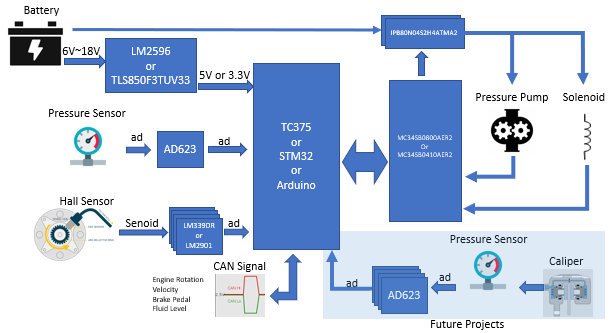
\includegraphics[width=0.8\textwidth]{figuras/arquitetura-funcional-do-sistema-de-controle-de-freio.png}
    \fonte{ O Autor.}
\end{figure}

\begin{comment}A Figura~\ref{fig:arquitetura-funcional-do-sistema-de-controle-de-freio} ilustra a arquitetura funcional do sistema de controle de freio com atuação digital embarcada. A placa de controle recebe sinais do pedal de freio, sensores de roda e do sistema ACC (Radar/Câmera), além de dados do módulo ECU do motor via barramento CAN. Com base nesses sinais, o microcontrolador processa as informações e gera comandos para a bomba eletro-hidráulica e válvulas solenoides, modulando a pressão do óleo aplicada aos freios de forma ajustável e responsiva.\end{comment}

A Figura~\ref{fig:arquitetura-funcional-do-sistema-de-controle-de-freio} ilustra a arquitetura funcional do sistema de controle de freio com atuação digital embarcada. A placa de controle recebe sinais do pedal de freio, sensores de roda e do sistema ACC (Radar/Câmera), além de dados do módulo ECU do motor via barramento CAN. Com base nesses sinais, o microcontrolador processa as informações e gera comandos tanto para as válvulas solenoides quanto para a bomba eletro-hidráulica, que é efetivamente acionada durante a modulação de pressão. Dessa forma, a pressão aplicada aos freios pode ser ajustada de maneira controlada e responsiva.

Cabe ressaltar que, apesar da integração proposta permitir a validação experimental das estratégias de controle digital, o escopo deste estudo está restrito ao ambiente simulado e controlado. Limitações inerentes à modelagem, à ausência de sensores adicionais e à simplificação dos atuadores devem ser consideradas na interpretação dos resultados. Futuras investigações poderão explorar a adoção de válvulas proporcionais, sensores de posição e estratégias de controle adaptativo para ampliar a robustez e a aplicabilidade do sistema em cenários reais.


%####################################################################
%####################################################################
%####################################################################
%####################################################################
\subsection{Definição das Variáveis}
\label{sec:controle-4-1-2}
\begin{comment}
Nesta etapa, são descritas as principais variáveis envolvidas na modelagem da dinâmica longitudinal do veículo, fundamentais para a análise e implementação do controle digital proposto. Algumas dessas grandezas são determinadas em níveis superiores do sistema ACC, como nos modelos de referência da MathWorks, mas desempenham papel central como entradas para o subsistema embarcado responsável pela atuação sobre os elementos hidráulicos.

\begin{itemize} 
    \item $x_e$: posição do veículo controlado [m] — representa a localização longitudinal do veículo sob análise. 
    \item $x_l$: posição do veículo líder [m] — indica a posição do veículo imediatamente à frente. 
    \item $v_e$: velocidade do veículo controlado [m/s] — velocidade instantânea do veículo sob controle. 
    \item $v_l$: velocidade do veículo líder [m/s] — velocidade do veículo à frente. 
    \item $d$: separação entre veículos [m] — distância relativa entre o veículo controlado e o líder. 
    \item $F_{\text{acc}}$: força resultante de tração ou frenagem [N] — força total aplicada ao veículo, seja para acelerar ou desacelerar. 
    \item $m$: massa total do veículo [kg] — parâmetro físico utilizado nos cálculos dinâmicos. 
    \item $c_r$: coeficiente de resistência ao movimento [N$\cdot$s/m] — engloba efeitos dissipativos, como atrito e arrasto aerodinâmico. 
\end{itemize}

No contexto do controle embarcado, o sistema recebe como sinais de entrada variáveis como $v_e$, $d$ e $v_{\text{rel}} = v_l - v_e$, processadas para o cálculo dos comandos PWM destinados à bomba de pressão e às válvulas solenoides. A pressão hidráulica nos cilindros das rodas é tratada como variável de saída do sistema, ajustada indiretamente por meio da corrente aplicada aos atuadores.

Embora esta abordagem contemple as principais variáveis tradicionalmente empregadas em modelagem veicular, outras grandezas podem ser incorporadas em estudos futuros, como temperatura do fluido, pressão atmosférica, ou parâmetros relacionados à aderência dos pneus, ampliando a fidelidade do modelo e a robustez das estratégias de controle.
\end{comment}

Esta subseção apresenta as variáveis fundamentais utilizadas no desenvolvimento do sistema de controle digital de frenagem. Embora algumas grandezas façam parte da dinâmica longitudinal do veículo, seu uso neste trabalho está limitado à geração dos sinais de referência provenientes do controlador ACC. A modelagem detalhada da dinâmica veicular não constitui o foco deste estudo, em vez disso, a ênfase recai sobre o comportamento hidráulico do sistema de freio e sobre a atuação dos componentes comandados pela placa de controle.

As principais variáveis consideradas são:

\begin{itemize}
    \item $x_e$: posição do veículo controlado [m] — utilizada apenas em níveis superiores do ACC.
    \item $x_l$: posição do veículo líder [m] — variável empregada na definição da separação entre veículos.
    \item $v_e$: velocidade do veículo controlado [m/s].
    \item $v_l$: velocidade do veículo líder [m/s].
    \item $d$: distância relativa entre veículos [m], calculada como $d = x_l - x_e$.
    \item $v_{\text{rel}} = v_l - v_e$: velocidade relativa, variável essencial para o cálculo da desaceleração desejada pelo ACC.
    \item $F_{\text{acc}}$: força longitudinal equivalente [N], mapeada em desaceleração desejada.
    \item $m$: massa total do veículo [kg].
    \item $c_r$: coeficiente equivalente de resistência ao movimento [N$\cdot$s/m], utilizado apenas para o cálculo conceitual de força longitudinal.
\end{itemize}

No contexto do presente trabalho, o controlador ACC fornece uma referência de desaceleração $a_{\text{des}}$, que é convertida em uma pressão hidráulica desejada $P_{\text{ref}}$. Esta pressão constitui a entrada do subsistema hidráulico modelado, sendo modulada pela atuação da bomba e das válvulas solenoides controladas via PWM. 

Assim, as variáveis descritas nesta seção têm papel auxiliar, servindo como interface entre o controlador de alto nível e o modelo hidráulico tratado nos capítulos seguintes. Variáveis adicionais, como temperatura do fluido, rigidez volumétrica ou condições de aderência, podem ser incorporadas em extensões futuras do modelo para aumentar sua fidelidade e robustez.

%####################################################################
%####################################################################
%####################################################################
%####################################################################
\subsection{Equações Dinâmicas}
\label{sec:controle-4-1-3}

A formulação matemática da dinâmica longitudinal do veículo é fundamental para a análise e implementação das estratégias de controle digital propostas neste estudo. O modelo adotado busca representar, de maneira simplificada, as principais forças atuantes durante a frenagem, considerando as limitações inerentes à abordagem embarcada e ao escopo experimental.

A variação temporal da velocidade do veículo controlado pode ser expressa por:

\begin{equation} \dot{v}e = \frac{1}{m} F{\text{acc}} - \frac{c_r}{m} v_e \end{equation}

Onde $\dot{v}e$ representa a aceleração longitudinal, $F{\text{acc}}$ corresponde à força resultante de tração ou frenagem, $m$ é a massa total do veículo e $c_r$ é o coeficiente de resistência ao movimento, que agrega efeitos como atrito e arrasto aerodinâmico.

A dinâmica da separação entre o veículo controlado e o veículo líder é descrita por:

\begin{equation} \dot{d} = v_l - v_e \end{equation}

Nesta expressão, $d$ indica a distância relativa, enquanto $v_l$ e $v_e$ são as velocidades do veículo líder e do veículo sob controle, respectivamente.

Para a definição da distância de seguimento desejada, adota-se uma relação linear com a velocidade, conforme sugerido por \citeonline{LuuAndLupu2019}:

\begin{equation} d_{ref} = r_0 + h \cdot v_e \end{equation}

Em que $r_0$ representa a distância mínima de segurança e $h$ o tempo de passagem.

No contexto do controle embarcado, a força de frenagem é implementada indiretamente por meio da modulação da pressão hidráulica nos cilindros das rodas. A relação entre a força de frenagem $F_{\text{brake}}$ e a pressão $P$ pode ser aproximada por:

%\begin{equation} F_{\text{brake}} = A_c \cdot P \end{equation}%

Com $A_c$ sendo a área efetiva do pistão do cilindro de freio. A pressão de referência necessária para atingir uma determinada desaceleração é estimada por:

\begin{equation} P_{\text{ref}} = \frac{m \cdot |a_{\text{des}}|}{A_c} \end{equation}

Onde $a_{\text{des}}$ é a aceleração desejada, definida pelo controlador de alto nível.


%####################################################################
%####################################################################
%####################################################################
%####################################################################
\subsubsection{Estimativa da Pressão de Frenagem e Controle Indireto}
\label{sec:controle-4-1-3-1}
Embora o modelo dinâmico apresentado anteriormente descreva a aceleração do veículo em função da força resultante $F_{\text{acc}}$, no contexto do controle embarcado, a placa de controle não atua diretamente sobre essa força. Em vez disso, ela modula a pressão hidráulica aplicada aos freios, a qual gera uma força de frenagem proporcional. Cabe destacar que a precisão na estimação da pressão de frenagem pode ser significativamente afetada pela evolução do coeficiente de atrito das lonas de freio, como discutido em \citeonline{ZhangWang2021}, sendo relevante considerar tais variações em aplicações práticas e em estratégias de controle indireto.

A relação entre a força de frenagem $F_{\text{brake}}$ e a pressão hidráulica $P$ pode ser aproximada por:

\begin{equation}
F_{\text{brake}} = A_c \cdot P
\end{equation}

Onde $A_c$ é a área efetiva do pistão do cilindro de freio.

Assumindo que a força de controle $F_{\text{acc}}$ desejada seja negativa (frenagem), podemos estimar a pressão necessária como:

\begin{equation}
P_{\text{ref}} = \frac{|F_{\text{acc}}|}{A_c} = \frac{m \cdot |a_{\text{des}}|}{A_c}
\end{equation}

Essa pressão de referência será utilizada como entrada para o subsistema de controle da placa, que deve gerar sinais para a bomba e válvulas solenoides para rastrear esse valor.

Este trabalho visa fazer o controle das válvulas solenoides do tipo ON/OFF, mas segundo  \citeonline{ChenLv2017}, a corrente necessária para atingir uma determinada pressão diferencial $\Delta p$ pode ser estimada pela equação:

\begin{equation}
i = \frac{\pi R_v^2 (\cos \alpha)^2}{K_i} \Delta p + \frac{K_s (x_0 + x_m)}{K_i}
\end{equation}

Onde:
\begin{itemize}
 \item $R_v$ é o raio da esfera da válvula,
 \item $\alpha$ é o ângulo do assento da válvula,
 \item $K_i$ é o coeficiente corrente-força,
 \item $K_s$ é a constante de rigidez da mola,
 \item $x_0$ é o pré-carregamento da mola,
 \item $x_m$ é o deslocamento máximo do êmbolo.
\end{itemize}

Essa corrente pode ser convertida em sinal PWM para controle das válvulas HSV e USV, conforme demonstrado experimentalmente por \citeonline{HouhuaJing2022}, que validaram a viabilidade de controle de pressão por modulação de ciclo de trabalho.  Estratégias similares de controle proporcional de pressão via PWM para atuadores de freio ABS também foram exploradas em \citeonline{ProportionalPressureABS2023}, evidenciando a eficácia do método em aplicações automotivas reais.

Portanto, e possível fazer uma estimação ainda melhor se levarmos em consideração o controle das válvulas solenoides, porem como foi dito, o controle da placa será baseado na conversão da aceleração desejada em pressão de referência, e desta em corrente ou PWM, permitindo o controle indireto da força de frenagem com alta precisão e robustez com o controle apenas da bomba de pressão.


\begin{comment}
    

%####################################################################
%####################################################################
%####################################################################
%####################################################################
\subsection{Modelo em Espaço de Estados do Subsistema Hidráulico}
\label{sec:controle-4-1-4}

Para descrever matematicamente o comportamento do subsistema hidráulico sob controle digital, adota-se uma modelagem em espaço de estados, que permite representar a evolução da pressão nos cilindros das rodas em função dos sinais de controle aplicados às válvulas solenoides. Esta abordagem é amplamente utilizada na literatura para análise e projeto de sistemas de controle embarcados, especialmente quando se busca compatibilidade com técnicas modernas, como LQR e observadores de estados.

A formulação parte da equação diferencial que relaciona a variação temporal da pressão hidráulica à atuação das válvulas, conforme apresentado por \citeonline{ChenLv2017}:

%\begin{equation} \frac{dp_w}{dt} = \frac{k_w}{A_w^2} C_d A_j \sqrt{\frac{2 \Delta p}{\rho}} \end{equation}%

Em que $p_w$ representa a pressão no cilindro da roda, $k_w$ é a rigidez do cilindro, $A_w$ a área da seção transversal, $C_d$ o coeficiente de descarga, $A_j$ a área efetiva da válvula (função do PWM aplicado), $\Delta p = p_m - p_w$ a diferença de pressão entre a bomba e o cilindro, e $\rho$ a densidade do fluido.

Considerando que o sinal de controle $u$ (PWM) pode ser relacionado linearmente à abertura da válvula, a equação pode ser reescrita como:

\begin{equation} \dot{p}_w = f(x, u) = \frac{k_w}{A_w^2} C_d \cdot \alpha \cdot u \cdot \sqrt{2(p_m - x)/\rho} \end{equation}

Onde $\dot{p}_w$ é o estado do sistema, $u$ é o comando PWM, e $\alpha$ representa o ganho proporcional entre o PWM e a área efetiva da válvula.

Embora o modelo seja inerentemente não linear, para fins de projeto de controladores digitais, é comum realizar a linearização em torno de um ponto de operação $(x_0, u_0)$. O sistema linearizado assume a forma:

\begin{equation} \dot{x} = a x + b u \end{equation}

Com os coeficientes $a$ e $b$ obtidos por derivação parcial de $f(x, u)$ em relação a $x$ e $u$, respectivamente.

Essa representação facilita a aplicação de técnicas de controle ótimo e observação de estados, além de permitir a análise de estabilidade e desempenho do subsistema hidráulico sob diferentes condições operacionais. A apesar da simplificação adotada, aspectos como não linearidades, histerese, variações térmicas e atrasos eletromecânicos não são explicitamente modelados nesta etapa, o que limita a abrangência dos resultados. Estratégias de identificação de parâmetros ou modelagem adaptativa podem ser consideradas em trabalhos futuros para ampliar a fidelidade do modelo.

A modelagem em espaço de estados proposta serve como base para o desenvolvimento e validação das estratégias de controle digital embarcado, viabilizando a simulação e análise do comportamento do sistema em diferentes cenários experimentais.
\end{comment}


%####################################################################
%####################################################################
%####################################################################
%####################################################################
\subsubsection{Simulação da Resposta da Pressão Hidráulica ao Sinal} \label{sec:controle-4-1-4-1}

A simulação da evolução da pressão hidráulica $p_w$ em função do sinal PWM aplicado à válvula constitui uma etapa fundamental para a análise do comportamento dinâmico do subsistema hidráulico sob diferentes condições de atuação. Para esse fim, a equação diferencial não linear que descreve a dinâmica da pressão foi discretizada utilizando o método de Euler explícito, permitindo a obtenção de uma aproximação numérica da resposta temporal do sistema.

\begin{equation} 
p_w(t + dt) = p_w(t) + \frac{dp_w}{dt} \cdot dt 
\end{equation}

Nesta abordagem, o termo $\frac{dp_w}{dt}$ é calculado a partir dos parâmetros físicos do sistema e do valor instantâneo do PWM, conforme estabelecido no modelo dinâmico. O procedimento adotado possibilita a avaliação da influência de diferentes ciclos de trabalho do PWM sobre a taxa de crescimento e o valor de equilíbrio da pressão hidráulica.

O código-fonte~\ref{cod:evolucao_pressao} em MATLAB apresentado a seguir implementa essa simulação para múltiplos valores de PWM, ilustrando a resposta do sistema ao longo do tempo:



A Figura~\ref{fig:Simulacao_da_Pressao_Hidraulica_com_PWM} apresenta os resultados obtidos, evidenciando a evolução da pressão para diferentes valores de PWM. Observa-se que ciclos de trabalho mais elevados resultam em uma elevação mais rápida da pressão, com tendência à estabilização em patamares superiores. O comportamento não linear do sistema é perceptível, especialmente nos instantes iniciais, refletindo a dependência da taxa de variação da pressão em relação à diferença de pressão disponível.

\begin{figure}[htbp]
    \centering
    \caption{Evolução da pressão hidráulica simulada para diferentes valores de PWM.}
    \label{fig:Simulacao_da_Pressao_Hidraulica_com_PWM}
    \includegraphics[width=0.8\textwidth]{figuras/Simulacao_da_Pressao_Hidraulica_com_PWM.png}
    \fonte{ O Autor.}
\end{figure}

Cabe destacar que, embora o método de Euler explícito seja amplamente utilizado pela sua simplicidade, outras técnicas numéricas, como \textit{Runge-Kutta}, podem ser empregadas para aprimorar a precisão da simulação, especialmente em sistemas com dinâmica mais complexa. Além disso, a análise de sensibilidade dos parâmetros físicos pode contribuir para a compreensão dos limites de atuação do modelo e para a calibração experimental do sistema.

Os resultados obtidos nesta etapa devem ser interpretados à luz das simplificações adotadas, servindo como referência para o ajuste dos algoritmos de controle digital e para a preparação de experimentos futuros em ambiente real.


%####################################################################
%####################################################################
%####################################################################
%####################################################################
\subsection{Parâmetros Numéricos do Subsistema Hidráulico}
\label{sec:controle-4-1-5}

A definição dos parâmetros físicos do subsistema hidráulico é fundamental para a modelagem, simulação e implementação do controle digital embarcado. Os valores adotados nesta etapa refletem especificações típicas encontradas na literatura e em componentes comerciais, servindo como referência inicial para a análise do comportamento dinâmico do sistema.

\begin{table}[h!] 
\Caption{\label{tab:parametros_hidraulico_formatado} Parâmetros do modelo hidráulico} 
\UNIFORtab{}{ 
    \begin{tabular}{ l | l | l } 
        \hline Parâmetro & Símbolo & Valor Típico \\ 
        \hline Pressão da bomba (entrada) & $p_m$ & $10 \times 10^6$ Pa \\ 
        \hline Densidade do fluido & $\rho$ & 850 kg/m³ \\ 
        \hline Área do cilindro da roda & $A_w$ & 0{,}002 m² \\ 
        \hline Rigidez do cilindro da roda & $k_w$ & 20000 N/m \\ 
        \hline Coeficiente de descarga da válvula & $C_d$ & 0{,}7 \\ 
        \hline Ganho PWM-área da válvula & $\alpha$ & $1 \times 10^{-6}$ m² \\ 
        \hline Ganho da válvula HSV & $\beta_1$ & 1{,}0 \\ 
        \hline Ganho da válvula USV & $\beta_2$ & 1{,}0 \\ 
        \hline Ganho da bomba & $\gamma$ & 1{,}0 \\ 
        \hline Ganho de realimentação & $\alpha$ & 0{,}1 \\ 
        \hline 
    \end{tabular} 
    }{     \Fonte{Elaborado pelo autor}     } 
\end{table}

Esses parâmetros podem ser ajustados conforme dados experimentais, recomendações de fabricantes ou resultados de identificação de sistemas. Sua escolha influencia diretamente a resposta dinâmica do modelo, a precisão das simulações e o desempenho dos algoritmos de controle.

É importante salientar que variações nesses valores, decorrentes de fatores como temperatura, desgaste de componentes, tolerâncias de fabricação ou condições ambientais, podem impactar significativamente o comportamento do sistema hidráulico. Trabalhos como o de \citeonline{ChenLv2017} destacam a necessidade de considerar tais incertezas, sugerindo o emprego de técnicas de controle robusto ou adaptativo para lidar com dispersões paramétricas e garantir desempenho satisfatório em diferentes cenários.

Por fim, a análise de sensibilidade dos parâmetros adotados pode contribuir para a calibração do modelo e para a definição de margens de segurança no projeto do controlador digital embarcado, além de orientar futuras investigações experimentais voltadas à validação do sistema em ambiente real.

%####################################################################
%####################################################################
%####################################################################
%####################################################################
\section{Simulação com Controle Preditivo (MPC)}
\label{sec:controle-4-1-6}

 Para avaliar o desempenho do sistema de controle digital embarcado, foi utilizado como referência o modelo Simulink \text{mpcACCsystem}, disponibilizado pela MathWorks \cite{Matlab2024}. Este modelo representa um cenário completo de ACC, no qual um controlador preditivo (MPC) determina o sinal de aceleração desejada ( a\_{\text{des}}(t) ) para o veículo ego, considerando a dinâmica do tráfego e as restrições de segurança.

Embora o foco deste trabalho não seja o desenvolvimento do controle MPC em si, a utilização desse modelo como gerador de sinais permite validar o subsistema de controle embarcada em condições próximas às encontradas em aplicações reais. A Figura~\ref{fig:simulink_model_for_lead_car_and_ego_car} ilustra a estrutura do modelo empregado.

\begin{figure}[htbp]
    \centering
    \caption{Modelo Simulink de ACC com MPC utilizado como gerador de sinais.}
    \label{fig:simulink_model_for_lead_car_and_ego_car}
    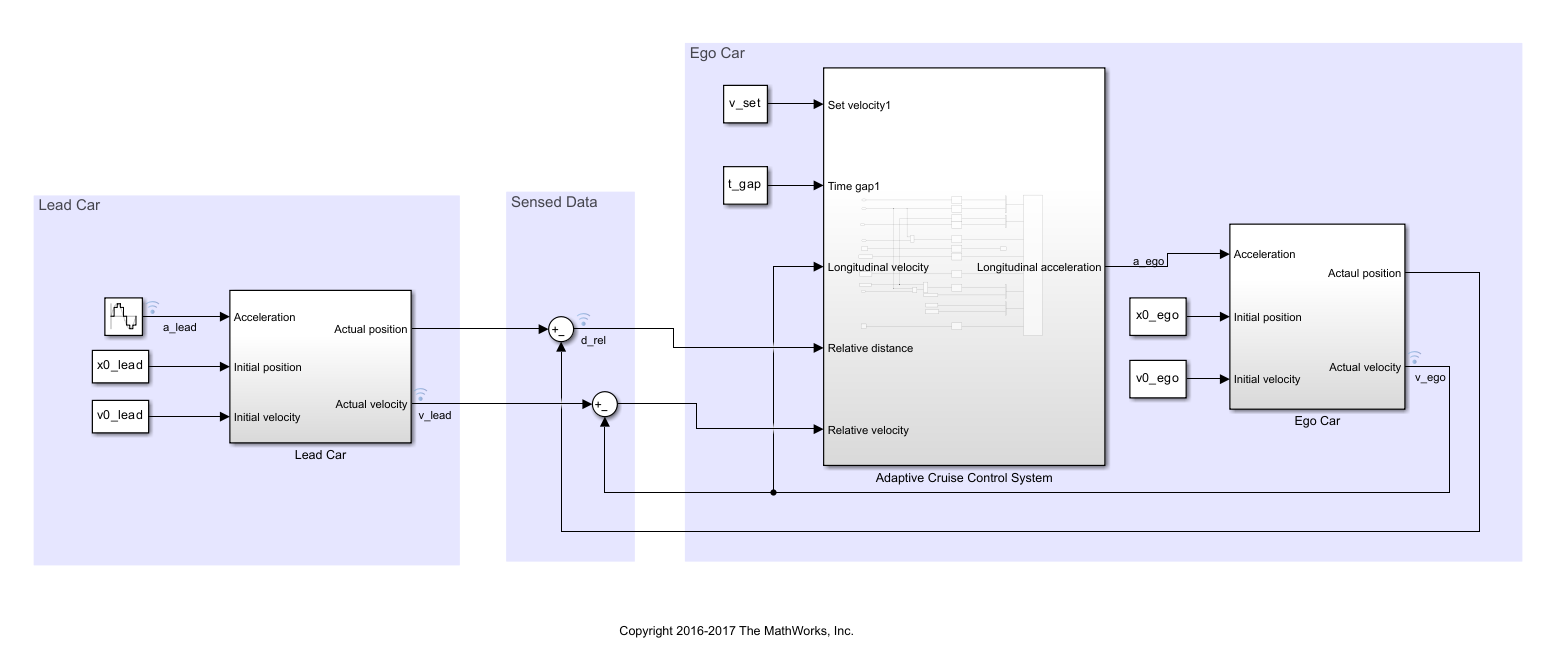
\includegraphics[width=0.8\textwidth]{figuras/simulink_model_for_lead_car_and_ego_car.png}
    \fonte{ O Autor adaptado de \cite{matwork-adaptive-cruise-control-using-model-predictive-controller}.}
\end{figure}

O sinal ( a\_{\text{des}}(t) ), produzido pelo bloco \textit{Adaptive Cruise Control System}, é empregado como entrada para um bloco \textit{MATLAB Function} que simula a resposta da pressão hidráulica do sistema de freio. Este bloco implementa a modelagem não linear da válvula hidráulica, conforme discutido anteriormente, e gera os sinais PWM correspondentes para a bomba e válvulas HSV/USV.

O código a seguir exemplifica a integração entre o controle preditivo e o subsistema hidráulico:

Essa integração possibilita analisar a coerência entre o controle de alto nível (ACC/MPC) e a atuação física do sistema de freio, demonstrando a viabilidade da arquitetura embarcada proposta. Os sinais de saída — pressão hidráulica, PWM da bomba e válvulas — são utilizados nas etapas seguintes para análise de desempenho e comparação com outras estratégias de controle. A Figura~\ref{fig:sinal_saida_bloco_controle_hidraulico_com_saida_modelo_acc_mcp} apresenta o comportamento do sistema sob diferentes condições de operação.

\begin{figure}[htbp]
    \centering
    %\caption{Sinal Saída Bloco Controle Hidráulico com Saída Modelo ACC MPC.}%
    \label{fig:sinal_saida_bloco_controle_hidraulico_com_saida_modelo_acc_mcp}
    \includegraphics[width=0.8\textwidth]{figuras/sinal_saida_bloco_controle_hidraulico_com_saida_modelo_acc_mcp.png}
    \fonte{ O Autor adaptado de \cite{Matlab2024}.}
\end{figure}


Apesar do modelo MPC permitir a consideração explícita de restrições e antecipação de comportamentos futuros, sua implementação embarcada demanda recursos computacionais significativos. Neste estudo, o MPC é utilizado apenas como referência para geração de sinais de teste, não sendo implementado diretamente no hardware. Futuras investigações poderão explorar a viabilidade de embarcar o controle preditivo, bem como avaliar o desempenho do sistema sob incertezas paramétricas e restrições operacionais mais rigorosas.


%####################################################################
%####################################################################
%####################################################################
%####################################################################
\section{Projeto do Controlador LQR}
\label{sec:controle-4-2}
O controle da pressão hidráulica no sistema de freio veicular embarcado demanda precisão, estabilidade e resposta adequada. Neste contexto, o Regulador Linear Quadrático (LQR) foi adotado como estratégia de controle digital, considerando sua capacidade de fornecer soluções ótimas para sistemas lineares e sua viabilidade computacional em aplicações embarcadas.

A literatura apresenta diversas alternativas para o controle de sistemas hidráulicos automotivos, incluindo abordagens baseadas em lógica difusa \cite{Pananurak2009}, controladores Proporcional-Integral (PI) \cite{YangYing2017}, Proporcional-Integral-Derivativo (PID) \cite{LuuAndLupu2019} e controle preditivo baseado em modelo (MPC) \cite{Tian2024, LihuaLuo2016}. Embora o MPC permita lidar com restrições e múltiplas variáveis, sua implementação em unidades de controle embarcadas pode ser limitada por requisitos computacionais elevados, decorrentes da necessidade de resolver problemas de otimização em tempo real, especialmente em plataformas com recursos restritos.

O LQR, por sua vez, oferece um compromisso entre desempenho e simplicidade, permitindo o projeto sistemático a partir de modelos linearizados, como o do subsistema hidráulico apresentado anteriormente. Sua aplicação possibilita a obtenção de sinais de controle suaves e estáveis, características desejáveis para evitar desgaste prematuro dos componentes e desconforto ao usuário.

A equação original do modelo hidráulico é dada por:

\begin{equation} \dot{p}_w = \frac{k_w}{A_w^2} C_d \cdot \alpha \cdot u \cdot \sqrt{\frac{2(p_m - p_w)}{\rho}} \end{equation}

A linearização em torno de um ponto de operação resulta nos coeficientes:

\begin{equation} a = \frac{\partial f}{\partial x} = -\frac{k_w}{A_w^2} C_d \alpha \sqrt{\frac{1}{2 \rho (p_m - p_w)}} \end{equation}

\begin{equation} b = \frac{\partial f}{\partial u} = \frac{k_w}{A_w^2} C_d \alpha \sqrt{\frac{2(p_m - p_w)}{\rho}} \end{equation}

Esses parâmetros são atualizados dinamicamente no bloco de controle, permitindo que o LQR se adapte às condições operacionais do sistema.

O controlador LQR busca minimizar a função de custo quadrática:

\begin{equation} J = \int_0^\infty (x^T Q x + u^T R u) dt \end{equation}

Os pesos ( Q ) e ( R ) podem ser ajustados segundo o erro de rastreamento e a pressão atual, promovendo maior robustez frente a variações de carga e dinâmica. Estratégias de ajuste automático desses pesos, ou mesmo a combinação com técnicas de controle robusto, podem ser consideradas em trabalhos futuros para lidar com incertezas mais pronunciadas.

O código a seguir exemplifica a implementação do controle LQR adaptativo para pressão hidráulica:

A Tabela~\ref{tab:parametros_lqr} apresenta os parâmetros físicos utilizados na simulação do controlador LQR:

\begin{table}[h!] 
\Caption{
\label{tab:parametros_lqr} Parâmetros físicos do subsistema hidráulico utilizados no controle LQR} 
\UNIFORtab{}{ 
    \begin{tabular}{ l | l | l | l } 
        \hline Parâmetro & Símbolo & Valor Típico & Unidade \\ 
        \hline Pressão da bomba (entrada) & $p_m$ & $10 \times 10^6$ & Pa \\ 
        \hline Densidade do fluido hidráulico & $\rho$ & 850 & kg/m³ \\ 
        \hline Área do cilindro da roda & $A_w$ & 0{,}002 & m² \\ 
        \hline Rigidez do cilindro da roda & $k_w$ & 20000 & N/m \\ 
        \hline Coeficiente de descarga da válvula & $C_d$ & 0{,}7 & — \\ 
        \hline Ganho PWM-área da válvula & $\alpha$ & $1 \times 10^{-6}$ & m² \\ 
        \hline 
    \end{tabular} }{ \Fonte{Elaborado pelo autor} } 
\end{table}

A aplicação do LQR ao subsistema hidráulico do sistema de freio veicular embarcado demonstrou-se adequada para os objetivos deste estudo, equilibrando desempenho, simplicidade de implementação e compatibilidade com sistemas embarcados. Futuras investigações podem explorar a integração com técnicas de controle robusto, modo deslizante (SMC) ou ajuste automático de parâmetros para ampliar a resiliência do sistema frente a incertezas e variações operacionais.

A Figura~\ref{fig:lqr_pressao_adaptativo_valvulas} demostra a aplicação do LQR ao subsistema hidráulico do sistema de freio veicular embarcado que se mostrou uma escolha adequada, equilibrando desempenho ótimo, simplicidade de implementação e compatibilidade com sistemas embarcados.

\begin{figure}[htbp]
    \centering
    \caption{Sinal Saída Bloco Controle Hidráulico com Saída Modelo ACC MPC.}
    \label{fig:lqr_pressao_adaptativo_valvulas}
    \includegraphics[width=0.8\textwidth]{figuras/lqr_pressao_adaptativo_valvulas.png}
    \fonte{ O Autor adaptado de \cite{Matlab2024}. }
\end{figure}

%Inclusive, a análise da literatura reforça essa decisão, destacando o LQR como uma alternativa eficiente frente a controladores clássicos e preditivos em contextos de controle digital da pressão indireta%.

%####################################################################
%####################################################################
%####################################################################
%####################################################################
%\section{Projeto do Observador de \textit{Luenberger}}%
\label{sec:controle-4-3}
Em sistemas embarcados de controle, nem sempre é possível medir diretamente todas as variáveis de estado relevantes para o desempenho do sistema. No contexto do controle da pressão hidráulica em sistemas de freio automotivo, sensores de pressão podem apresentar limitações, como ruído, atrasos ou até mesmo falhas intermitentes. Diante dessas restrições, a estimação de estados internos a partir de medições disponíveis torna-se uma estratégia fundamental para aumentar a confiabilidade e robustez do controle.

O Observador de \textit{Luenberger} é uma abordagem clássica e amplamente utilizada para estimar variáveis de estado em sistemas lineares, especialmente quando se dispõe de um modelo matemático razoavelmente preciso. Considerando o modelo linearizado do subsistema hidráulico, o observador pode ser descrito pelas seguintes equações:

\begin{equation}
\dot{x} = a x + b u, \quad y = c x
\end{equation}

Onde:
\begin{itemize}
 \item \( x = p_w \): pressão no cilindro da roda (estado do sistema)
 \item \( u \): sinal PWM aplicado à válvula
 \item \( y \): pressão medida (com ruído)
 \item \( a, b \): coeficientes do modelo linearizado
 \item \( c = 1 \): saída diretamente proporcional ao estado
\end{itemize}

O observador de \textit{Luenberger} é implementado como:

\begin{equation}
\dot{\hat{x}} = a \hat{x} + b u + L(y - \hat{y}), \quad \hat{y} = c \hat{x}
\end{equation}

O termo ( $L(y - \hat{y})$) representa a realimentação do erro de estimação, ajustando a dinâmica do observador para que a estimativa ( $\hat{x}$ ) possa convergir ao valor real de ( $x$ ). O ganho ( $L$ ) é escolhido de modo que o erro de estimação ( $e = x - \hat{x}$ ) seja capaz de evoluir de acordo com:

\begin{equation}
\dot{e} = (a - Lc)e
\end{equation}

A seleção adequada de ( $L$ ) é essencial para garantir a convergência e a estabilidade do observador, sendo comumente realizada por alocação de polos ou técnicas de otimização. Em aplicações práticas, a escolha do ganho pode ser influenciada por fatores como ruído de medição, incertezas paramétricas e requisitos de resposta dinâmica.

O exemplo a seguir, Código~\ref{cod:observador_luenberger},ilustra a implementação do observador de \textit{Luenberger} em MATLAB:



A simulação do observador deve evidenciar: 
\begin{itemize} 
    \item Convergência da estimativa ( $\hat{x}$ ) para o valor real de ( $x$ ) mesmo na presença de ruído. 
    \item Robustez frente a variações do sinal PWM e perturbações na medição. 
    \item Estabilidade da estimação ao longo do tempo. 
\end{itemize}

A Figura~\ref{fig:observador_pressao_luenberger} apresenta o desempenho do observador de \textit{Luenberger} na estimação da pressão hidráulica em tempo real.

\begin{figure}[htbp]
    \centering
    \caption{Sinal Saída Bloco Controle Hidráulico com Saída Modelo ACC MPC.}
    \label{fig:observador_pressao_luenberger}
    \includegraphics[width=0.8\textwidth]{figuras/observador_pressao_luenberger.png}
    \fonte{ O Autor adaptado de \cite{Matlab2024}. }
\end{figure}

Embora o Observador de \textit{Luenberger} seja uma solução eficiente para sistemas lineares, alternativas como o filtro de Kalman ou observadores robustos podem ser consideradas em cenários com maior incerteza, ou não linearidades acentuadas. A escolha da técnica de estimação deve levar em conta as características do sistema, a disponibilidade de sensores e os requisitos de desempenho da aplicação.

%####################################################################
%####################################################################
%####################################################################
%####################################################################
%\section{Validação Experimental e Integração Final}%
\label{sec:controle-4-4}

Após o desenvolvimento dos modelos matemáticos, do projeto do controlador LQR e da implementação do observador de \textit{Luenberger}, esta seção apresenta a simulação integrada do sistema embarcado de controle de freio com ACC. O objetivo é avaliar a integração dos blocos funcionais e examinar o desempenho do sistema no rastreamento da pressão hidráulica de referência, considerando aspecto de precisão e estabilidade.

A simulação contempla os seguintes blocos conectados sequencialmente:

\begin{itemize} 
    \item \textbf{ACC (Adaptive Cruise Control)}: responsável pela geração do sinal de aceleração desejada \(a_{\text{des}}\) a partir da distância e velocidade relativa ao veículo à frente. 
    \item \textbf{Conversor (\(a_{\text{des}} \rightarrow p_{w,\text{ref}}\))}: realiza a conversão da aceleração desejada em pressão hidráulica de referência, conforme a relação: 
          \[ p_{w,\text{ref}} = \frac{m \cdot a_{\text{des}}}{A_c} \] 
    \item \textbf{Controlador LQR Adaptativo}: determina o sinal PWM necessário para rastrear \(p_{w,\text{ref}}\), utilizando o modelo linearizado atualizado em tempo real. 
    \item \textbf{Observador de \textit{Luenberger}}: estima a pressão real \(\hat{p}_w\) a partir do sinal PWM e da pressão medida, contribuindo para a mitigação de ruídos e atrasos. 
    \item \textbf{Modelo Hidráulico}: simula a evolução da pressão real \(p_w\) em função do sinal PWM aplicado. 
\end{itemize}

A simulação integrada busca:

\begin{itemize} 
    \item Verificar a capacidade do sistema em rastrear a pressão hidráulica de referência derivada de \(a_{\text{des}}\). 
    \item Avaliar a suavidade e a estabilidade do sinal PWM gerado pelo controlador. 
    \item Analisar o erro de estimação entre \(p_w\) e \(\hat{p}_w\) ao longo do tempo. 
\end{itemize}

O Código~\ref{cod:controle_integrado} a seguir representa o núcleo da simulação embarcada, integrando o controlador LQR adaptativo e o observador de \textit{Luenberger}:

A simulação deve ser executada em um laço temporal (por exemplo, em um \textit{script Simulink} ou MATLAB), onde a cada passo de tempo:

\begin{enumerate}
 \item O modelo ACC fornece \(a_{\text{des}}\).
 \item Calcula-se \(p_{w,\text{ref}}\).
 \item O bloco \textbf{controle\_integrado} é chamado com os parâmetros do sistema.
 \item As saídas PWM, \(\hat{p}_w\) e \(\text{erro}_{\text{est}}\) são armazenadas para análise.
\end{enumerate}

A Figura~\ref{fig:controle_integrado_lqr_luenberger} apresenta a simulação integrada e permite validar o comportamento do sistema de controle embarcado em condições realistas. A arquitetura modular facilita a substituição de blocos por versões físicas (sensores reais, atuadores, etc.) em futuras etapas de implementação. Os resultados obtidos com essa simulação são fundamentais para comprovar a viabilidade do controle digital da pressão hidráulica em sistemas de freio com ACC.

\begin{figure}[htbp]
    \centering
    \caption{Sinal Saída Bloco Controle Hidráulico com Saída Modelo ACC MPC.}
    \label{fig:controle_integrado_lqr_luenberger}
    \includegraphics[width=0.8\textwidth]{figuras/controle_integrado_lqr_luenberger.png}
    \fonte{ O Autor adaptado de \cite{Matlab2024}. }
\end{figure}


%####################################################################
%####################################################################
%####################################################################
%####################################################################
\section{Análise de Robustez do Sistema de Controle}
\label{sec:controle-4-5}

Após o desenvolvimento dos modelos matemáticos, do projeto do controlador LQR e da implementação do observador de \textit{Luenberger}, esta seção apresenta a simulação integrada do sistema embarcado de controle de freio com ACC. O objetivo é avaliar a integração dos blocos funcionais e examinar o desempenho do sistema no rastreamento da pressão hidráulica de referência, considerando aspecto de precisão e estabilidade.

A simulação contempla os seguintes blocos conectados sequencialmente:

\begin{itemize} 
    \item \textbf{ACC (Adaptive Cruise Control)}: responsável pela geração do sinal de aceleração desejada \(a_{\text{des}}\) a partir da distância e velocidade relativa ao veículo à frente. 
    \item \textbf{Conversor (\(a_{\text{des}} \rightarrow p_{w,\text{ref}}\))}: realiza a conversão da aceleração desejada em pressão hidráulica de referência, conforme a relação: 
          \[ p_{w,\text{ref}} = \frac{m \cdot a_{\text{des}}}{A_c} \] 
    \item \textbf{Controlador LQR Adaptativo}: determina o sinal PWM necessário para rastrear \(p_{w,\text{ref}}\), utilizando o modelo linearizado atualizado em tempo real. 
    \item \textbf{Observador de \textit{Luenberger}}: estima a pressão real \(\hat{p}_w\) a partir do sinal PWM e da pressão medida, contribuindo para a mitigação de ruídos e atrasos. 
    \item \textbf{Modelo Hidráulico}: simula a evolução da pressão real \(p_w\) em função do sinal PWM aplicado. 
\end{itemize}

A simulação integrada busca:

\begin{itemize} 
    \item Verificar a capacidade do sistema em rastrear a pressão hidráulica de referência derivada de \(a_{\text{des}}\). 
    \item Avaliar a suavidade e a estabilidade do sinal PWM gerado pelo controlador. 
    \item Analisar o erro de estimação entre \(p_w\) e \(\hat{p}_w\) ao longo do tempo. 
\end{itemize}

O Código~\ref{cod:controle_integrado} a seguir representa o núcleo da simulação embarcada, integrando o controlador LQR adaptativo e o observador de \textit{Luenberger}:



A execução da simulação ocorre em um laço temporal, no qual, a cada iteração:

\begin{enumerate} 
\item O modelo ACC fornece \(a_{\text{des}}\). 
\item Calcula-se ($ p_{w,\text{ref}}$ ). 
\item O bloco \textbf{controle\_integrado} é chamado com os parâmetros do sistema. 
\item As saídas ( $PWM$ ), ( $\hat{p}w$ ) e ($ erro{est}$ ) são armazenadas para análise posterior. 
\end{enumerate}

A Figura~\ref{fig:controle_robusto_simulink} que apresenta os resultados da simulação integrada, permite avaliar o comportamento do sistema de controle embarcado em condições próximas às reais. A arquitetura modular adotada facilita a substituição de blocos por versões físicas (sensores e atuadores reais) em etapas futuras, bem como a integração com plataformas HIL para validação experimental mais abrangente.

\begin{figure}[htbp]
    \centering
    \caption{Sinal Saída Bloco Controle Hidráulico com Saída Modelo ACC MPC.}
    \label{fig:controle_robusto_simulink}
    \includegraphics[width=0.8\textwidth]{figuras/controle_robusto_simulink.png}
    \fonte{ O Autor adaptado de \cite{Matlab2024}. }
\end{figure}

Cabe ressaltar que, embora a simulação forneça evidências da viabilidade da abordagem proposta, limitações inerentes ao ambiente computacional e à modelagem adotada devem ser consideradas na interpretação dos resultados. Fatores como latência de sensores, ruído eletromagnético e tolerâncias de fabricação não são plenamente capturados nesta etapa. Futuras investigações poderão explorar a validação experimental em hardware real, bem como a análise de desempenho sob diferentes cenários operacionais e perturbações externas.


%####################################################################
%####################################################################
%####################################################################
%####################################################################
\section{Discussão Crítica} 
\label{cap:discussao_critica}

O desenvolvimento de um sistema de controle digital embarcado para o freio veicular com ACC representa um avanço relevante na interface entre teoria de controle, eletrônica embarcada e segurança automotiva. Contudo, como em todo projeto aplicado, é fundamental analisar criticamente as premissas, simplificações e limitações inerentes à abordagem adotada.

A modelagem do subsistema hidráulico, ainda que fundamentada em referências consolidadas, parte do pressuposto de linearidade em torno de pontos de operação e desconsidera efeitos não lineares mais complexos, como histerese das válvulas, variações térmicas do fluido, atrasos eletromecânicos e a evolução do coeficiente de atrito das lonas de freio.

Já estudos recentes sugerem que a consideração dinâmica desse coeficiente pode aprimorar a precisão da estimação da pressão de frenagem, especialmente em sistemas sujeitos a desgaste e variações operacionais \cite{ZhangWang2021}. Além disso, pesquisas sobre o projeto paramétrico de motores em sistemas de freio eletro-hidráulicos reforçam a importância de integrar modelagem precisa e validação experimental para garantir desempenho otimizado em aplicações reais \cite{MotorParametricDesign2023}. Essas simplificações foram necessárias para viabilizar a implementação em tempo real no microcontrolador automotivo, mas restringem a precisão do modelo em situações extremas ou sob condições operacionais variáveis.

A escolha do controlador LQR mostrou-se adequada do ponto de vista computacional e de desempenho para sistemas lineares. Sua capacidade de fornecer soluções ótimas com baixo esforço de controle e estabilidade é compatível com aplicações embarcadas. No entanto, o desempenho do LQR depende fortemente da qualidade da linearização e da seleção dos pesos $Q$ e $R$, que aqui foram ajustados de forma heurística.

 Em cenários com variações abruptas de carga ou parâmetros, pode haver degradação do desempenho, o que justifica a consideração de estratégias adaptativas ou robustas em projetos posteriores. Estratégias de controle coordenado de pressão, como as propostas em \cite{PressureCoordinatedControl2023}, têm se mostrado eficazes para lidar com essas variações e garantir maior robustez ao sistema de frenagem eletro-hidráulico.

A implementação do observador de \textit{Luenberger} contribuiu para a robustez do sistema, permitindo a estimação da pressão hidráulica mesmo na presença de ruído ou falhas de sensores. Entretanto, o observador pressupõe conhecimento preciso dos parâmetros do modelo, o que pode não se confirmar em ambiente real. A sensibilidade do ganho $L$ à localização dos polos do observador também requer atenção, pois ajustes inadequados podem comprometer a estabilidade da estimação. Alternativas como o filtro de Kalman ou observadores robustos podem ser exploradas para lidar com incertezas paramétricas e ruídos não gaussianos.

Outro aspecto relevante é a ausência de validação em hardware real. Embora as simulações em MATLAB/Simulink tenham demonstrado a coerência do modelo e a viabilidade do controle, a transição para um ambiente físico envolve desafios adicionais, como latência de sensores, ruído eletromagnético, tolerâncias de fabricação e falhas intermitentes. A integração com sensores reais, como radar e câmera do sistema ADAS, também não foi abordada nesta etapa, embora seja fundamental para a operação completa do ACC.

A arquitetura modular proposta, com separação clara entre controle de alto nível ACC e controle de baixo nível (pressão hidráulica), mostrou-se alinhada com práticas contemporâneas de engenharia de sistemas embarcados. Essa modularidade facilita a substituição de blocos por versões mais sofisticadas, como controladores preditivos MPC, técnicas de controle robusto ou observadores não lineares, sem comprometer a estrutura do sistema. Além disso, a adoção de plataformas HIL pode ser considerada para validação experimental mais abrangente, aproximando ainda mais o estudo das condições reais de operação.





\begin{comment}
\textbf{\textit{Everton sugere que como o trabalho sera feito em modelagem, que faca o detalhamento da modelagem mecânica do modelo de freio, capitulo estimativa de presa de frenagem e controle indireto. }}

    \subsection{Estimativa da Pressão de Frenagem}
\label{sec:controle-estimacao-pressao}

Embora o sistema conte com um sensor de pressão instalado no bloco hidráulico, a medição disponível reflete apenas a pressão na linha principal, não necessariamente a pressão efetiva na câmara de cada freio. Além disso, a presença de ruído, atraso de amostragem e quantização exige que o controlador utilize não apenas o valor medido, mas também uma estimativa dinâmica da pressão.

A dinâmica da pressão no freio pode ser descrita em função das vazões de entrada e saída, controladas pelas válvulas solenoides, e da atuação da bomba eletro-hidráulica. Dessa forma, a pressão instantânea pode ser aproximada por modelos baseados em balanço de massa e compressibilidade do fluido. Este modelo permite inferir a pressão na câmara do freio mesmo em intervalos em que a válvula está comutada ou quando o sensor apresenta comportamento ruidoso.

Assim, o sistema de controle utiliza uma combinação entre a pressão medida e a pressão estimada pelo modelo hidráulico. Essa estimativa é especialmente importante em situações de variações rápidas da demanda de frenagem, comuns em aplicações de ACC, nas quais a bomba precisa modular a pressão de forma contínua. A fusão entre o sinal medido e a estimativa permite reduzir o impacto de ruído e melhorar a estabilidade do controlador.


###########################################################################
##############################################################################
##############################################################################3
##########################################################################3

Perfeito, Elton — vamos **pegar o capítulo do jeito que está** e **organizar** para chegar exatamente onde você quer **sem sair gerando texto agora**. Vou te entregar:

1.  **Mapa de corte/manutenção** (o que fica e o que sai, já na ordem final)
2.  **Arquitetura do capítulo “Controle” reorganizada** (só títulos + 1–2 frases guia por item)
3.  **Esqueleto LaTeX pronto para colar** (com seções, labels e *placeholders*), incluindo **onde inserir a sua planta** (equações do `Bloco_Hidraulico`) e **onde usar o MPC como gerador de referência**
4.  **Checklist de pendências mínimas** (para cada bloco, o que precisa existir para a banca “enxergar” coerência)
5.  **Onde mover o que for secundário** (Apêndice)

***

## 1) O que manter, o que retirar (corte cirúrgico)

**Manter (com pequenos ajustes de ligação):**

*   **Introdução** do capítulo (primeiros parágrafos do ACC e escopo).
*   **Seção “Modelagem da Planta”** — mas **agora ela vai, de fato, apresentar a planta** (seu modelo `Bloco_Hidraulico`).
*   **Seção “Simulação com Controle Preditivo (MPC)”** — como **gerador de $$a_{\text{des}}(t)$$**, não como controlador embarcado.

**Retirar por ora (ou mover para apêndice/futuros trabalhos):**

*   LQR, Observador de Luenberger, Análise de Robustez, Tabelas/Figuras relativas a esses blocos e qualquer “placeholder de código” não preenchido.
*   “Tabela de Distâncias ACC” (se quiser manter, **mover para Introdução/Estado da Arte** ou usar **apenas como saturação do $$a_{\text{des}}$$** com 1 linha explicativa).

***

## 2) Arquitetura do capítulo “Controle” (versão enxuta e coerente)

> **Objetivo**: mostrar **(i)** a planta hidráulica que você REALMENTE usa, **(ii)** como o ACC/MPC gera a **referência de aceleração**, **(iii)** como você **converte para referência de pressão** e **(iv)** como a planta responde.  
> (Sem entrar ainda em LQR/observador.)

**Cap. Controle – índice proposto**

1.  **Introdução** *(manter, só ajustar 1 frase de escopo)*  
    – “Este capítulo apresenta a **planta hidráulica modelada**, o **mapeamento $$a_{\text{des}}\to p_{\text{ref}}$$** e os **ensaios de simulação** com o ACC/MPC como gerador de sinais.”

2.  **Modelagem da Planta** *(agora com a planta de fato)*  
    2.1 **Hipóteses e arquitetura hidráulica** (duas linhas: fluido compressível, câmara equivalente, válvulas *inlet/outlet*, bomba, reservatório)  
    2.2 **Equações do subsistema hidráulico** *(do seu `Bloco_Hidraulico`)*  
    – Balanceamento de volumes/pressão (compressibilidade):
    $$
    \dot P=\frac{\beta}{V}\big(Q_b+Q_{\text{in}}-Q_{\text{out}}-K_{\text{leak}}\,P\big)
    $$
    – Bomba (função de $$\omega_p$$ e contrapressão): $$Q_b(\omega_p,P)$$  
    – Válvulas como orifícios:
    $$
    Q_{\text{in}}=C_{v,\text{in}}A_{\text{in,max}}u_{\text{in}}\sqrt{\tfrac{2\,\max(P_{\text{sup}}-P,0)}{\rho}},\quad
    Q_{\text{out}}=C_{v,\text{out}}A_{\text{out,max}}u_{\text{out}}\sqrt{\tfrac{2\,\max(P-P_{\text{ret}},0)}{\rho}}
    $$
    – Pressão a montante $$P_{\text{sup}}$$ (reservatório / mestre / manifold pressurizado pela bomba).  
    2.3 **Sinais de controle e saturações** (definir domínios: $$u_{\text{in}},u_{\text{out}}\in[0,1]$$, $$\omega_p\ge0$$).  
    2.4 **Parâmetros de simulação** *(tabela curta; rotular como “parâmetros de simulação”, não “típicos”)*  
    2.5 **Onde fica o código** *(indicar Apêndice com a listagem da função)*

3.  **Conversor $$a_{\text{des}} \rightarrow p_{\text{ref}}$$**  
    – Apresentar **a ponte**: usar sua forma simples **explicitando** que é aproximação de cilindro equivalente:
    $$
    p_{\text{ref}}=\kappa\,\frac{m\,|a_{\text{des}}|}{A_{\text{eq}}}
    $$
    com nota de que $$\kappa$$ é fator de calibração (pode incorporar distribuição por eixo, raio efetivo e atrito).  
    – **Limites/saturações** (p. ex. $$0\le p_{\text{ref}}\le p_{\max}$$).

4.  **Simulação com ACC/MPC como gerador de referência** *(manter sua seção, mas com foco)*  
    – Citar o modelo `mpcACCsystem` (MathWorks) **apenas como fonte de $$a_{\text{des}}(t)$$**.  
    – Diagrama simples: $$a_{\text{des}}(t)$$$$\rightarrow$$ conversor $$\rightarrow p_{\text{ref}}(t)$$$$\rightarrow$$ **planta hidráulica** $$\rightarrow P(t)$$.  
    – **Cenários de teste** (3 curtos):
    *   S1: degrau de $$a_{\text{des}}$$ (–0.5 m/s²)
    *   S2: rampa (–0→–1 m/s² em 2 s)
    *   S3: pulso (–1 m/s² por 0.5 s)  
        – **Métricas**: tempo de subida 10–90%, tempo de acomodação, *tracking error* $$|P-P_{\text{ref}}|$$ (mesmo que em malha “quase aberta”, dá para avaliar coerência do modelo).

5.  **Resultados e discussão curta (plant response)**  
    – 1–2 gráficos: $$P(t)$$ vs $$p_{\text{ref}}(t)$$ para S1–S3 (legendas com parâmetros).  
    – 1 parágrafo: “onde o modelo atende / onde satura” (p.ex., limitação por $$Q_b$$, $$A_{\text{in}}$$, etc.).  
    – **Limitações**: sem controle fechado ainda; controle será foco de trabalho futuro (ou capítulo subsequente).

6.  **Limitações e próximos passos**  
    – Enumerar o que entra depois: PI/LQR, observador/estimador, validação HIL; considerar histerese de válvulas, temperatura do fluido.

**Apêndice**

*   **Listagem da função `Bloco_Hidraulico`** (com `\lstlisting` ou verbatim), e um mini-*README* dos parâmetros.
*   Se quiser, **diagramas Simulink** (prints) em apêndice também.

***

## 3) Esqueleto LaTeX (pronto para colar e preencher aos poucos)

> **Obs.:** É um esqueleto enxuto para você ajustar localmente. Onde escrevi “(preencher)”, basta pôr 2–3 linhas.

```latex
% ======================
\chapter{Metodologia Específica: Controle Digital Para um Sistema de Freio ACC}
\label{cap:controle}

% --- 1. Introdução (MANTER, só ajustar 1 linha final de escopo)
% (seu texto atual)
% Acrescente ao final:
% Este capítulo apresenta a planta hidráulica modelada, o mapeamento a_des -> p_ref e os ensaios de simulação com ACC/MPC como gerador de sinais.

% --- 2. Modelagem da Planta
\section{Modelagem da Planta}
\label{sec:controle-planta}

\subsection{Hipóteses e Arquitetura}
\label{sec:planta-hipoteses}
% (preencher) Fluido compressível (módulo β), volume equivalente V, válvulas inlet/outlet como orifícios, bomba acionada por ω_p, reservatório a P_ret, ponto de suprimento P_sup.

\subsection{Equações do Subsistema Hidráulico}
\label{sec:planta-equacoes}

\noindent\textbf{Balanço de compressibilidade:}
\begin{equation}
\dot P = \frac{\beta}{V}\,\big(Q_b + Q_{\text{in}} - Q_{\text{out}} - K_{\text{leak}}\,P\big).
\end{equation}

\noindent\textbf{Bomba (fonte de vazão com perda):}
\begin{equation}
Q_b = K_b\,\omega_p - K_{lb}\,P,\qquad Q_b \ge 0.
\end{equation}

\noindent\textbf{Válvulas como orifícios equivalentes:}
\begin{align}
Q_{\text{in}} &= C_{v,\text{in}} A_{\text{in,max}} u_{\text{in}} \sqrt{\frac{2\,\max(P_{\text{sup}}-P,0)}{\rho}},\\
Q_{\text{out}}&= C_{v,\text{out}}A_{\text{out,max}} u_{\text{out}}\sqrt{\frac{2\,\max(P-P_{\text{ret}},0)}{\rho}}.
\end{align}

\noindent\textbf{Pressão a montante da inlet:}
% (preencher brevemente)
% P_sup = P_ret + K_sup * (ω_p / 2π), limitado por P_sup,max  (ou outras arquiteturas)

\subsection{Sinais de Controle e Saturações}
\label{sec:planta-controle}
% (preencher) u_in, u_out ∈ [0,1], ω_p ≥ 0; políticas simples: por ora, perfis prescritos nos ensaios.

\subsection{Parâmetros de Simulação}
\label{sec:planta-parametros}
% (preencher) tabela pequena (β, V, ρ, P_ret, K_b, K_lb, C_v,in/out, A_in/out,max, K_sup, P_sup,max).
% Rotular como "Parâmetros de simulação". Fonte: calibração do autor.

\subsection{Listagem do Modelo}
\label{sec:planta-listagem}
A implementação computacional do modelo hidráulico encontra-se no Apêndice~\ref{ap:bloco-hidraulico}, sob a função \texttt{Bloco\_Hidraulico}.

% --- 3. Conversor a_des -> p_ref
\section{Conversão de Aceleração para Referência de Pressão}
\label{sec:controle-conversor}

\noindent\textbf{Relação de referência (cilindro equivalente):}
\begin{equation}
p_{\text{ref}}(t) = \kappa\,\frac{m\,|a_{\text{des}}(t)|}{A_{\text{eq}}},\qquad 0 \le p_{\text{ref}} \le p_{\max}.
\end{equation}
% (preencher 2 linhas) Nota sobre κ (calibração) e A_eq (área equivalente / distribuição por eixo).

% --- 4. Simulação com ACC/MPC (manter sua seção, porém focada)
\section{Simulação com Controle Preditivo (MPC)}
\label{sec:controle-mpc}
% (seu texto) Ajustar para: MPC da MathWorks utilizado como gerador de a_des(t).
% Inserir 3 cenários (S1, S2, S3) e métricas (rise time, settling, erro |P - p_ref|).

% --- 5. Resultados
\section{Resultados e Discussão}
\label{sec:controle-resultados}
% (preencher) 1-2 figuras com P(t) vs p_ref(t) nos cenários S1..S3 com legendas contendo parâmetros.

% --- 6. Limitações e Próximos Passos
\section{Limitações e Próximos Passos}
\label{sec:controle-limites}
% (preencher) listar ausência de malha fechada real, histerese de válvulas, temperatura, estimador; próximos passos: PI/LQR, observador, HIL, etc.

% --- Apêndice com a função
\appendix
\section{Listagem do Modelo Hidráulico (\texttt{Bloco\_Hidraulico})}
\label{ap:bloco-hidraulico}
% \lstinputlisting[language=Matlab]{Bloco_Hidraulico.m}
% ou colar como verbatim, se preferir
```

> **Observação:** Se você já usa um arquivo `.m`, recomendo `\lstinputlisting` (pacote `listings`) para manter sempre sincronizado.

***

## 4) Checklist mínimo por bloco (para “passar na banca”)

*   **Modelagem da Planta**  
    ☐ Equações **explícitas** (as mesmas da função)  
    ☐ Tabela **pequena** de parâmetros (com a palavra “simulação”)  
    ☐ Vínculo claro de símbolos ↔ variáveis do código (e.g., $$K_b \leftrightarrow$$ `Kb`)  
    ☐ Referência ao **Apêndice** onde está a função

*   **Conversor $$a_{\text{des}}\to p_{\text{ref}}$$**  
    ☐ Equação **curta** com $$\kappa$$ (calibração)  
    ☐ **Saturações** (limites de pressão)

*   **Simulação com ACC/MPC**  
    ☐ Dizer que o MPC é **apenas gerador de sinais**  
    ☐ Definir **3 cenários** e **métricas**  
    ☐ Gráficos com **legendas informativas** (parâmetros)

*   **Resultados**  
    ☐ Pelo menos **2 figuras** $$P(t)$$ vs $$p_{\text{ref}}(t)$$  
    ☐ 1 parágrafo **curto** explicando comportamento e limitações

*   **Apêndice**  
    ☐ Listagem do `Bloco_Hidraulico`  
    ☐ (Opcional) Print do diagrama Simulink do pipeline

***

## 5) Onde colocar o que sobrou (sem apagar seu trabalho)

*   **LQR, Observador, Robustez** → criar **Seção “Trabalhos Futuros”** (ou manter títulos comentados e citar no fim como roadmap).
*   “Tabela de Distâncias ACC” → **Introdução/Estado da Arte** ou **nota de saturação** no conversor (1 linha).

***

### Quer que eu monte **a Tabela de Parâmetros** já no formato LaTeX (com os seus nomes de variáveis do código) e um **mini-mapa de símbolos** (código ↔ equação) para colar em \S\ref{sec:planta-parametros}?

Se disser “sim”, eu te devolvo **só esses dois blocos prontos**, sem gerar texto extra.



######################################################################################
ELTON******************************************************************************
*********************************************************************************
##############################################################################################


######################################################################################
ELTON******************************************************************************
*********************************************************************************
##############################################################################################



######################################################################################
ELTON******************************************************************************
*********************************************************************************
##############################################################################################



######################################################################################
ELTON******************************************************************************
*********************************************************************************
##############################################################################################



######################################################################################
ELTON******************************************************************************
*********************************************************************************
##############################################################################################










% !TeX root = ../documento.tex
\chapter{Metodologia Específica: Controle Digital Para um Sistema de Freio ACC}
\label{cap:controle}

O Controle de Cruzeiro Adaptativo (ACC) constitui uma tecnologia relevante nos veículos modernos, especialmente em contextos de direção assistida e autônoma. Sua principal função é ajustar automaticamente a velocidade do veículo para manter uma distância segura em relação ao veículo à frente, promovendo conforto, segurança e eficiência no trânsito.


Embora existam diversas abordagens teóricas para o desenvolvimento de sistemas ACC, a aplicação prática ainda apresenta desafios consideráveis. Muitos trabalhos concentram-se em simulações e modelagens teóricas, enquanto a implementação em hardware embarcado permanece menos explorada na literatura.

Neste estudo, busca-se contribuir para essa lacuna ao propor e validar um sistema de controle digital para o freio veicular com base em ACC, utilizando o microcontrolador automotivo AURIX TC375. O desenvolvimento inclui uma placa de controle dedicada, modelagem do sistema em espaço de estados e a aplicação de técnicas de controle digital. A validação é realizada por meio de simulações no MATLAB/Simulink e testes práticos em ambiente controlado, visando analisar a viabilidade da solução em condições representativas.

O sistema proposto foi desenvolvido para: 
\begin{itemize} 
    \item Investigar a capacidade de manter a distância segura em relação ao veículo à frente; 
    \item Avaliar o controle da pressão de frenagem de forma precisa e responsiva; 
    \item Explorar a implementação em hardware real, com sensores e atuadores automotivos. 
\end{itemize}

A Figura~\ref{fig:Acc_tabela_de_distancias} apresenta uma tabela que relaciona a distância de relativa $d$, a desaceleração $a$, e a velocidade relativa máxima $v_{\text{rel}}$ que pode ser compensada com segurança, conforme a equação:

\begin{equation}
v_{\text{rel}} = -\sqrt{2d \cdot a}
\end{equation}

Essa expressão, derivada sob a hipótese de desaceleração uniforme e trajetória retilínea, fornece um limite operacional para o ACC em situações de aproximação rápida. Dessa forma, a tabela serve como referência para definir valores seguros de desaceleração a serem empregadas na geração do sinal $a_{\text{des}}$ utilizado nas simulações subsequentes.

\begin{figure}[htbp]
    \centering
    \caption{Tabela de Distâncias para o Sistema ACC}
    \label{fig:Acc_tabela_de_distancias}
    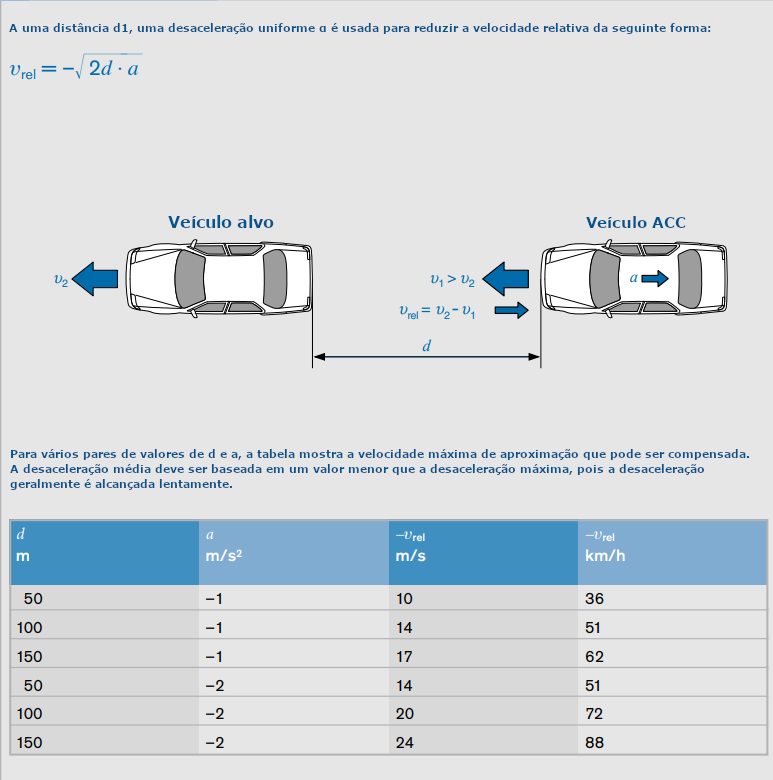
\includegraphics[width=0.8\textwidth]{figuras/Acc_tabela_de_distancias.png}
    \fonte{ O Autor, adaptado de \cite{Konrad2014}.}
\end{figure}
\begin{comment}
    A solução é manter a figura, mas explicar seu papel:
ela define o limite operacional de segurança do ACC, servindo para limitar o comando de desaceleração enviado ao controlador hidráulico mais adiante.
\end{comment}

Enquanto muitos estudos abordam o ACC sob a ótica de simulações e modelagens teóricas, este trabalho busca avançar na direção de uma solução prática, com implementação em um sistema embarcado. A escolha do microcontrolador AURIX TC375 fundamenta-se em sua robustez, capacidade de processamento e conformidade com normas de segurança automotiva (ISO 26262 - ASIL-D).

Cabe ressaltar que o escopo deste estudo está restrito à validação do sistema em ambiente simulado e controlado, reconhecendo-se limitações inerentes à experimentação laboratorial, à modelagem adotada e à ausência de testes em condições reais de operação. Os resultados obtidos devem ser interpretados como subsídio para investigações futuras e não como solução definitiva para aplicações industriais.


%####################################################################
%####################################################################
%####################################################################
%####################################################################
\section{Modelagem da Planta}
\label{sec:controle-4-1}

O objetivo desta seção é apresentar a modelagem da planta do sistema de frenagem, com ênfase na atuação da placa de controle digital sobre os componentes do módulo hidráulico — especificamente, as válvulas solenoides e a bomba de pressão. O comportamento do sistema ACC é utilizado como cenário de aplicação, mas o foco principal está na implementação prática do controle embarcado.

Em veículos modernos, a arquitetura \textit{brake-by-wire} (freio por fio) e a substituição de conexões mecânicas por atuadores eletrônicos têm possibilitado maior integração com sistemas de controle embarcados. Essa abordagem é relevante para a implementação de estratégias de frenagem ativa, como o ACC, e tem sido objeto de investigação em veículos experimentais \cite{Pananurak2009}.

Neste trabalho, optou-se por uma modelagem simplificada da dinâmica longitudinal do veículo, suficiente para validar a estratégia de controle digital proposta e a atuação da placa desenvolvida. Embora existam modelos mais completos na literatura, que incluem motor, conversor de torque, transmissão e rodas \cite{LuuAndLupu2019}, tais abordagens demandam maior complexidade computacional e não constituem o foco deste estudo.

A arquitetura hierárquica do ACC pode ser dividida em dois níveis: um controlador de alto nível, responsável por calcular a aceleração desejada (por exemplo, via \textit{Model Predictive Control} - MPC), e um controlador de baixo nível, que executa os comandos nos atuadores. Essa estrutura, conforme descrito por \citeonline{Tian2024}, pode contribuir para a estabilidade e segurança do sistema em tempo real.

Para representar a lógica de comutação entre acelerador e freio, abordagens como a modelagem \textit{Mixed Logical Dynamical} (MLD) são utilizadas na literatura \cite{LihuaLuo2016}, permitindo capturar o comportamento híbrido do sistema ACC. No entanto, neste estudo, adota-se uma modelagem contínua simplificada, considerada suficiente para os objetivos de validação da estratégia de controle digital e da placa desenvolvida.

No contexto do sistema de frenagem, a precisão na modulação da pressão hidráulica é um aspecto central. Pesquisas como a de \citeonline{ChenLv2017} propõem o uso de válvulas de comutação com controle linear da queda de pressão, enquanto \citeonline{HouhuaJing2022} destaca o uso de válvulas do tipo \textit{High-Speed Valve} (HSV) e \textit{Unload Solenoid Valve} (USV), controladas por modulação por largura de pulso (PWM) para ajuste da pressão nos cilindros das rodas. Recentemente, métodos de controle coordenado de pressão foram propostos para sistemas eletro-hidráulicos, visando melhorar a resposta dinâmica e a robustez do sistema de freio, conforme apresentado em \citeonline{PressureCoordinatedControl2023} e \citeonline{ProportionalPressureABS2023}.

Dessa forma, a modelagem adotada neste projeto considera a dinâmica longitudinal do veículo, com ênfase na atuação da placa de controle sobre os atuadores hidráulicos. A placa desenvolvida é responsável por gerar sinais para controlar as válvulas, além de acionar a bomba de pressão. Essa arquitetura permite modular a pressão de frenagem de maneira ajustável, dentro das limitações do modelo e do ambiente experimental.

Cabe ressaltar que, embora a modelagem proposta seja fundamentada em referências consolidadas, ela incorpora simplificações necessárias para viabilizar a implementação em ambiente embarcado e simulado. \begin{comment} Aspectos como não linearidades complexas, histerese das válvulas, variações térmicas do fluido e atrasos eletromecânicos não são explicitamente considerados neste estágio, o que limita a abrangência dos resultados.\end{comment} Aspectos como não linearidades complexas, variações térmicas do fluido, compressibilidade dependente da temperatura e atrasos eletromecânicos dos atuadores não são explicitamente considerados neste estágio. Tais efeitos, reconhecidos na literatura como mais significativos para a dinâmica do sistema do que a histerese individual das válvulas, são deixados para estudos futuros que possam aprofundar a análise em maior detalhe. Assim, os resultados apresentados devem ser interpretados como uma contribuição incremental para o entendimento e validação de estratégias de controle digital em sistemas de frenagem automotiva.


%####################################################################
%####################################################################
%####################################################################
%####################################################################
\subsection{Integração com Atuadores Hidráulicos}
\label{sec:controle-4-1-1}

A atuação sobre os componentes hidráulicos do sistema de freio foi estruturada a partir de duas abordagens complementares, amplamente discutidas na literatura:

\begin{itemize} 
    \begin{comment}        
    \item \textbf{Modulação linear da queda de pressão:} conforme proposto por\citeonline{ChenLv2017}, é possível controlar a pressão de saída da válvula com base na corrente aplicada à bobina, operando no estado crítico de equilíbrio da válvula. Essa técnica permite um controle mais preciso da pressão utilizando válvulas do tipo ON/OFF (atuadores eletromecânicos binários), embora válvulas proporcionais também possam ser consideradas em estudos futuros para maior flexibilidade de atuação. 
    \end{comment}
    \item \textbf{Modulação linear da queda de pressão:} conforme discutido em \citeonline{ChenLv2017}, válvulas ON/OFF podem apresentar uma relação aproximadamente linear entre a queda de pressão e a corrente aplicada à bobina quando operam no estado crítico de equilíbrio. No presente trabalho, essa referência é utilizada apenas como fundamentação teórica, uma vez que a estratégia proposta não implementa diretamente o método completo de modulação linear apresentado pelos autores.
    \item \textbf{Controle ativo por PWM:} como demonstrado por \citeonline{HouhuaJing2022}, válvulas do tipo High-Speed Valve (HSV) e Unload Solenoid Valve (USV) podem ser controladas por sinais PWM para ajustar a taxa de pressurização e despressurização nos cilindros das rodas. Essa abordagem possibilita um controle dinâmico e adaptativo da pressão durante a frenagem ativa, sendo compatível com a arquitetura embarcada proposta neste trabalho. 
\end{itemize}

Além dessas estratégias, a literatura recente destaca o uso de sensores de posição e pressão para realimentação do sistema, permitindo a implementação de malhas fechadas de controle mais robustas \cite{HouhuaJingShihao2023}. Embora o presente estudo tenha adotado uma abordagem baseada em controle indireto via PWM, a integração de sensores adicionais pode ser considerada em etapas futuras para aprimorar a precisão e a confiabilidade do sistema.

A placa de controle desenvolvida neste projeto foi configurada para permitir a implementação dessas estratégias, possibilitando a comutação entre modos de controle conforme a necessidade do sistema e os requisitos experimentais.

\begin{figure}[htbp]
    \centering
    \caption{Arquitetura geral do sistema de controle de freio ACC com microcontrolador embarcado}
    \label{fig:arquitetura-funcional-do-sistema-de-controle-de-freio}
    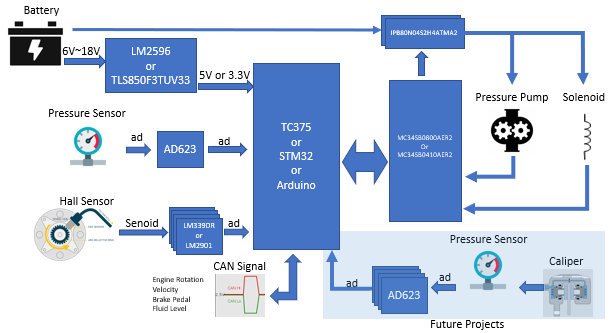
\includegraphics[width=0.8\textwidth]{figuras/arquitetura-funcional-do-sistema-de-controle-de-freio.png}
    \fonte{ O Autor.}
\end{figure}

\begin{comment}A Figura~\ref{fig:arquitetura-funcional-do-sistema-de-controle-de-freio} ilustra a arquitetura funcional do sistema de controle de freio com atuação digital embarcada. A placa de controle recebe sinais do pedal de freio, sensores de roda e do sistema ACC (Radar/Câmera), além de dados do módulo ECU do motor via barramento CAN. Com base nesses sinais, o microcontrolador processa as informações e gera comandos para a bomba eletro-hidráulica e válvulas solenoides, modulando a pressão do óleo aplicada aos freios de forma ajustável e responsiva.\end{comment}

A Figura~\ref{fig:arquitetura-funcional-do-sistema-de-controle-de-freio} ilustra a arquitetura funcional do sistema de controle de freio com atuação digital embarcada. A placa de controle recebe sinais do pedal de freio, sensores de roda e do sistema ACC (Radar/Câmera), além de dados do módulo ECU do motor via barramento CAN. Com base nesses sinais, o microcontrolador processa as informações e gera comandos tanto para as válvulas solenoides quanto para a bomba eletro-hidráulica, que é efetivamente acionada durante a modulação de pressão. Dessa forma, a pressão aplicada aos freios pode ser ajustada de maneira controlada e responsiva.

Cabe ressaltar que, apesar da integração proposta permitir a validação experimental das estratégias de controle digital, o escopo deste estudo está restrito ao ambiente simulado e controlado. Limitações inerentes à modelagem, à ausência de sensores adicionais e à simplificação dos atuadores devem ser consideradas na interpretação dos resultados. Futuras investigações poderão explorar a adoção de válvulas proporcionais, sensores de posição e estratégias de controle adaptativo para ampliar a robustez e a aplicabilidade do sistema em cenários reais.


%####################################################################
%####################################################################
%####################################################################
%####################################################################
\subsection{Definição das Variáveis}
\label{sec:controle-4-1-2}
\begin{comment}
Nesta etapa, são descritas as principais variáveis envolvidas na modelagem da dinâmica longitudinal do veículo, fundamentais para a análise e implementação do controle digital proposto. Algumas dessas grandezas são determinadas em níveis superiores do sistema ACC, como nos modelos de referência da MathWorks, mas desempenham papel central como entradas para o subsistema embarcado responsável pela atuação sobre os elementos hidráulicos.

\begin{itemize} 
    \item $x_e$: posição do veículo controlado [m] — representa a localização longitudinal do veículo sob análise. 
    \item $x_l$: posição do veículo líder [m] — indica a posição do veículo imediatamente à frente. 
    \item $v_e$: velocidade do veículo controlado [m/s] — velocidade instantânea do veículo sob controle. 
    \item $v_l$: velocidade do veículo líder [m/s] — velocidade do veículo à frente. 
    \item $d$: separação entre veículos [m] — distância relativa entre o veículo controlado e o líder. 
    \item $F_{\text{acc}}$: força resultante de tração ou frenagem [N] — força total aplicada ao veículo, seja para acelerar ou desacelerar. 
    \item $m$: massa total do veículo [kg] — parâmetro físico utilizado nos cálculos dinâmicos. 
    \item $c_r$: coeficiente de resistência ao movimento [N$\cdot$s/m] — engloba efeitos dissipativos, como atrito e arrasto aerodinâmico. 
\end{itemize}

No contexto do controle embarcado, o sistema recebe como sinais de entrada variáveis como $v_e$, $d$ e $v_{\text{rel}} = v_l - v_e$, processadas para o cálculo dos comandos PWM destinados à bomba de pressão e às válvulas solenoides. A pressão hidráulica nos cilindros das rodas é tratada como variável de saída do sistema, ajustada indiretamente por meio da corrente aplicada aos atuadores.

Embora esta abordagem contemple as principais variáveis tradicionalmente empregadas em modelagem veicular, outras grandezas podem ser incorporadas em estudos futuros, como temperatura do fluido, pressão atmosférica, ou parâmetros relacionados à aderência dos pneus, ampliando a fidelidade do modelo e a robustez das estratégias de controle.
\end{comment}

Esta subseção apresenta as variáveis fundamentais utilizadas no desenvolvimento do sistema de controle digital de frenagem. Embora algumas grandezas façam parte da dinâmica longitudinal do veículo, seu uso neste trabalho está limitado à geração dos sinais de referência provenientes do controlador ACC. A modelagem detalhada da dinâmica veicular não constitui o foco deste estudo, em vez disso, a ênfase recai sobre o comportamento hidráulico do sistema de freio e sobre a atuação dos componentes comandados pela placa de controle.

As principais variáveis consideradas são:

\begin{itemize}
    \item $x_e$: posição do veículo controlado [m] — utilizada apenas em níveis superiores do ACC.
    \item $x_l$: posição do veículo líder [m] — variável empregada na definição da separação entre veículos.
    \item $v_e$: velocidade do veículo controlado [m/s].
    \item $v_l$: velocidade do veículo líder [m/s].
    \item $d$: distância relativa entre veículos [m], calculada como $d = x_l - x_e$.
    \item $v_{\text{rel}} = v_l - v_e$: velocidade relativa, variável essencial para o cálculo da desaceleração desejada pelo ACC.
    \item $F_{\text{acc}}$: força longitudinal equivalente [N], mapeada em desaceleração desejada.
    \item $m$: massa total do veículo [kg].
    \item $c_r$: coeficiente equivalente de resistência ao movimento [N$\cdot$s/m], utilizado apenas para o cálculo conceitual de força longitudinal.
\end{itemize}

No contexto do presente trabalho, o controlador ACC fornece uma referência de desaceleração $a_{\text{des}}$, que é convertida em uma pressão hidráulica desejada $P_{\text{ref}}$. Esta pressão constitui a entrada do subsistema hidráulico modelado, sendo modulada pela atuação da bomba e das válvulas solenoides controladas via PWM. 

Assim, as variáveis descritas nesta seção têm papel auxiliar, servindo como interface entre o controlador de alto nível e o modelo hidráulico tratado nos capítulos seguintes. Variáveis adicionais, como temperatura do fluido, rigidez volumétrica ou condições de aderência, podem ser incorporadas em extensões futuras do modelo para aumentar sua fidelidade e robustez.

%####################################################################
%####################################################################
%####################################################################
%####################################################################
\subsection{Equações Dinâmicas}
\label{sec:controle-4-1-3}

A formulação matemática da dinâmica longitudinal do veículo é fundamental para a análise e implementação das estratégias de controle digital propostas neste estudo. O modelo adotado busca representar, de maneira simplificada, as principais forças atuantes durante a frenagem, considerando as limitações inerentes à abordagem embarcada e ao escopo experimental.

A variação temporal da velocidade do veículo controlado pode ser expressa por:

\begin{equation} \dot{v}e = \frac{1}{m} F{\text{acc}} - \frac{c_r}{m} v_e \end{equation}

Onde $\dot{v}e$ representa a aceleração longitudinal, $F{\text{acc}}$ corresponde à força resultante de tração ou frenagem, $m$ é a massa total do veículo e $c_r$ é o coeficiente de resistência ao movimento, que agrega efeitos como atrito e arrasto aerodinâmico.

A dinâmica da separação entre o veículo controlado e o veículo líder é descrita por:

\begin{equation} \dot{d} = v_l - v_e \end{equation}

Nesta expressão, $d$ indica a distância relativa, enquanto $v_l$ e $v_e$ são as velocidades do veículo líder e do veículo sob controle, respectivamente.

Para a definição da distância de seguimento desejada, adota-se uma relação linear com a velocidade, conforme sugerido por \citeonline{LuuAndLupu2019}:

\begin{equation} d_{ref} = r_0 + h \cdot v_e \end{equation}

Em que $r_0$ representa a distância mínima de segurança e $h$ o tempo de passagem.

No contexto do controle embarcado, a força de frenagem é implementada indiretamente por meio da modulação da pressão hidráulica nos cilindros das rodas. A relação entre a força de frenagem $F_{\text{brake}}$ e a pressão $P$ pode ser aproximada por:

%\begin{equation} F_{\text{brake}} = A_c \cdot P \end{equation}%

Com $A_c$ sendo a área efetiva do pistão do cilindro de freio. A pressão de referência necessária para atingir uma determinada desaceleração é estimada por:

\begin{equation} P_{\text{ref}} = \frac{m \cdot |a_{\text{des}}|}{A_c} \end{equation}

Onde $a_{\text{des}}$ é a aceleração desejada, definida pelo controlador de alto nível.


%####################################################################
%####################################################################
%####################################################################
%####################################################################
\subsubsection{Estimativa da Pressão de Frenagem e Controle Indireto}
\label{sec:controle-4-1-3-1}
Embora o modelo dinâmico apresentado anteriormente descreva a aceleração do veículo em função da força resultante $F_{\text{acc}}$, no contexto do controle embarcado, a placa de controle não atua diretamente sobre essa força. Em vez disso, ela modula a pressão hidráulica aplicada aos freios, a qual gera uma força de frenagem proporcional. Cabe destacar que a precisão na estimação da pressão de frenagem pode ser significativamente afetada pela evolução do coeficiente de atrito das lonas de freio, como discutido em \citeonline{ZhangWang2021}, sendo relevante considerar tais variações em aplicações práticas e em estratégias de controle indireto.

A relação entre a força de frenagem $F_{\text{brake}}$ e a pressão hidráulica $P$ pode ser aproximada por:

\begin{equation}
F_{\text{brake}} = A_c \cdot P
\end{equation}

Onde $A_c$ é a área efetiva do pistão do cilindro de freio.

Assumindo que a força de controle $F_{\text{acc}}$ desejada seja negativa (frenagem), podemos estimar a pressão necessária como:

\begin{equation}
P_{\text{ref}} = \frac{|F_{\text{acc}}|}{A_c} = \frac{m \cdot |a_{\text{des}}|}{A_c}
\end{equation}

Essa pressão de referência será utilizada como entrada para o subsistema de controle da placa, que deve gerar sinais para a bomba e válvulas solenoides para rastrear esse valor.

Este trabalho visa fazer o controle das válvulas solenoides do tipo ON/OFF, mas segundo  \citeonline{ChenLv2017}, a corrente necessária para atingir uma determinada pressão diferencial $\Delta p$ pode ser estimada pela equação:

\begin{equation}
i = \frac{\pi R_v^2 (\cos \alpha)^2}{K_i} \Delta p + \frac{K_s (x_0 + x_m)}{K_i}
\end{equation}

Onde:
\begin{itemize}
 \item $R_v$ é o raio da esfera da válvula,
 \item $\alpha$ é o ângulo do assento da válvula,
 \item $K_i$ é o coeficiente corrente-força,
 \item $K_s$ é a constante de rigidez da mola,
 \item $x_0$ é o pré-carregamento da mola,
 \item $x_m$ é o deslocamento máximo do êmbolo.
\end{itemize}

Essa corrente pode ser convertida em sinal PWM para controle das válvulas HSV e USV, conforme demonstrado experimentalmente por \citeonline{HouhuaJing2022}, que validaram a viabilidade de controle de pressão por modulação de ciclo de trabalho.  Estratégias similares de controle proporcional de pressão via PWM para atuadores de freio ABS também foram exploradas em \citeonline{ProportionalPressureABS2023}, evidenciando a eficácia do método em aplicações automotivas reais.

Portanto, e possível fazer uma estimação ainda melhor se levarmos em consideração o controle das válvulas solenoides, porem como foi dito, o controle da placa será baseado na conversão da aceleração desejada em pressão de referência, e desta em corrente ou PWM, permitindo o controle indireto da força de frenagem com alta precisão e robustez com o controle apenas da bomba de pressão.


%####################################################################
%####################################################################
%####################################################################
%####################################################################
\subsection{Modelo hidráulico em duas pressões ($P_{sup}$ e $P_w$)}
\label{sec:controle-modelo-hidraulico-2p}

Para o subsistema hidráulico, adota-se uma representação concentrada (\textit{lumped parameter}) com duas regiões de compressibilidade equivalentes: (i) uma região de suprimento/manifold, caracterizada pela pressão $P_{sup}$, associada ao volume efetivo $V_{sup}$ e ao retorno a baixa pressão $P_{ret}$; e (ii) um canal equivalente de roda (linha/caliper), caracterizado pela pressão $P_w$ e pelo volume efetivo $V_w$. Essa estrutura é compatível com a arquitetura de moduladores ABS/EHB, na qual a bomba fornece energia hidráulica ao suprimento e as válvulas determinam a transferência e o alívio de pressão no canal.

As dinâmicas das pressões são obtidas a partir da equação da continuidade para fluido compressível, resultando em:

\begin{equation}
\dot{P}_{sup}(t) = \frac{\beta}{V_{sup}}\left(Q_{pump}(t) - Q_{in}(t) - Q_{leak,sup}(t)\right),
\label{eq:psup_dot}
\end{equation}

\begin{equation}
\dot{P}_{w}(t) = \frac{\beta}{V_{w}}\left(Q_{in}(t) - Q_{out}(t) - Q_{leak,w}(t)\right),
\label{eq:pw_dot}
\end{equation}

onde $\beta$ é o módulo volumétrico efetivo do fluido e $Q_{pump}$, $Q_{in}$ e $Q_{out}$ representam, respectivamente, a vazão fornecida pela bomba, a vazão através da válvula de entrada (do suprimento para o canal) e a vazão através da válvula de saída (do canal para o retorno).

\subsubsection{Bomba e vazamentos internos}
\label{sec:controle-bomba-2p}

A bomba é modelada por uma relação linear simplificada entre vazão e velocidade angular do motor, com um termo de vazamento interno proporcional ao diferencial de pressão em relação ao retorno:

\begin{equation}
Q_{pump}(t) = K_b\,\omega_p(t) - K_{lb}\left(P_{sup}(t) - P_{ret}\right),
\label{eq:qpump_2p}
\end{equation}

em que $\omega_p$ é a velocidade angular do motor da bomba e $K_b$ e $K_{lb}$ são parâmetros equivalentes do conjunto motor--bomba.

\subsubsection{Válvulas e lei do orifício}
\label{sec:controle-valvulas-2p}

As vazões pelas válvulas de entrada e saída são representadas por uma lei de orifício, com abertura efetiva proporcional ao comando PWM normalizado ($0\leq u \leq 1$):

\begin{equation}
Q_{in}(t) = C_{v,in}\,A_{in,\max}\,u_{in}(t)\,\sqrt{\frac{2\,\max\left(P_{sup}(t)-P_w(t),\,0\right)}{\rho}},
\label{eq:qin_2p}
\end{equation}

\begin{equation}
Q_{out}(t) = C_{v,out}\,A_{out,\max}\,u_{out}(t)\,\sqrt{\frac{2\,\max\left(P_{w}(t)-P_{ret},\,0\right)}{\rho}},
\label{eq:qout_2p}
\end{equation}

onde $\rho$ é a densidade do fluido, $C_{v,in}$ e $C_{v,out}$ são coeficientes equivalentes de descarga, e $A_{in,\max}$ e $A_{out,\max}$ representam áreas máximas efetivas. O operador $\max(\cdot,0)$ garante consistência física (sem vazões imaginárias) quando os diferenciais de pressão se invertem.

Para fins de simulação, pode-se ainda incluir vazamentos equivalentes $Q_{leak,sup}$ e $Q_{leak,w}$ (proporcionais a $P_{sup}-P_{ret}$ e $P_w-P_{ret}$, respectivamente), representando relaxamento de pressão, permeabilidade e microvazamentos.

\subsection{Ensaios em malha aberta com degraus (validação do modelo)}
\label{sec:controle-ensaio-malha-aberta}

Antes do projeto em malha fechada, realiza-se a validação do modelo em malha aberta por meio de entradas em degrau nos atuadores, visando verificar causalidade, saturações e coerência física das variáveis internas ($Q_{pump}$, $Q_{in}$ e $Q_{out}$). Nesta etapa, a pressão é analisada preferencialmente em termos de pressão \textit{gauge} em bar, dada por:

\begin{equation}
P_{g}(t) = \frac{P(t)-P_{ret}}{10^5}\ \ [\text{bar}].
\label{eq:pressao_gauge_bar}
\end{equation}

\subsubsection{Teste 1: pressurização (bomba + válvula de entrada)}
\label{sec:controle-teste1}

No Teste 1, fixa-se $u_{in}=1$ e $u_{out}=0$, e aplica-se uma sequência de degraus na velocidade da bomba $\omega_p(t)$. Espera-se que $P_{sup}$ e $P_w$ aumentem em patamares e que, devido à válvula de saída permanecer fechada, a pressão no canal $P_w$ tenda a se manter próxima ao patamar atingido quando $\omega_p$ retorna a zero. Esse comportamento é coerente com a presença de fluido aprisionado no volume $V_w$ na ausência de caminho de descarga e/ou vazamento equivalente.

\subsubsection{Teste 2: alívio de pressão (válvula de saída)}
\label{sec:controle-teste2}

No Teste 2, estabelece-se inicialmente um patamar de pressão (por exemplo, utilizando o Teste 1) e, em seguida, fixa-se $\omega_p=0$ e $u_{in}=0$, aplicando-se degraus em $u_{out}$. Espera-se uma redução monotônica de $P_w$ em direção a $P_{ret}$, com $Q_{out}$ apresentando comportamento compatível com a lei do orifício.

\subsubsection{Teste 3: restrição de entrada (variação de $u_{in}$)}
\label{sec:controle-teste3}

No Teste 3, fixa-se $u_{out}=0$ e utiliza-se um valor constante de $\omega_p$ para manter o suprimento pressurizado, aplicando-se degraus em $u_{in}$. Este ensaio permite avaliar a influência da restrição de entrada na taxa de pressurização do canal e ajustar os parâmetros efetivos $C_{v,in}A_{in,\max}$.

\subsubsection{Parâmetros iniciais e escala de vazões}
\label{sec:controle-parametros-iniciais-ensaio}

Para que os ensaios em malha aberta produzam respostas fisicamente coerentes (evitando que $Q_{in}$ seja ordens de grandeza maior do que $Q_{pump}$), os parâmetros efetivos das válvulas devem ser compatíveis com a vazão disponível da bomba no ponto de operação. Na prática, isso implica ajustar $A_{in,\max}$ e $A_{out,\max}$ de modo que $Q_{in}$ e $Q_{out}$ tenham a mesma ordem de grandeza de $Q_{pump}$ durante os degraus de $\omega_p$. Nesta pesquisa, os testes iniciais mostraram coerência ao utilizar áreas efetivas reduzidas (por exemplo, $A_{in,\max}=A_{out,\max}=10^{-7}\ \text{m}^2$) como ponto de partida, com ajustes subsequentes baseados nos sinais observados.


\begin{comment}
    

%####################################################################
%####################################################################
%####################################################################
%####################################################################
\subsection{Modelo em Espaço de Estados do Subsistema Hidráulico}
\label{sec:controle-4-1-4}

Para descrever matematicamente o comportamento do subsistema hidráulico sob controle digital, adota-se uma modelagem em espaço de estados, que permite representar a evolução da pressão nos cilindros das rodas em função dos sinais de controle aplicados às válvulas solenoides. Esta abordagem é amplamente utilizada na literatura para análise e projeto de sistemas de controle embarcados, especialmente quando se busca compatibilidade com técnicas modernas, como LQR e observadores de estados.

A formulação parte da equação diferencial que relaciona a variação temporal da pressão hidráulica à atuação das válvulas, conforme apresentado por \citeonline{ChenLv2017}:

%\begin{equation} \frac{dp_w}{dt} = \frac{k_w}{A_w^2} C_d A_j \sqrt{\frac{2 \Delta p}{\rho}} \end{equation}%

Em que $p_w$ representa a pressão no cilindro da roda, $k_w$ é a rigidez do cilindro, $A_w$ a área da seção transversal, $C_d$ o coeficiente de descarga, $A_j$ a área efetiva da válvula (função do PWM aplicado), $\Delta p = p_m - p_w$ a diferença de pressão entre a bomba e o cilindro, e $\rho$ a densidade do fluido.

Considerando que o sinal de controle $u$ (PWM) pode ser relacionado linearmente à abertura da válvula, a equação pode ser reescrita como:

\begin{equation} \dot{p}_w = f(x, u) = \frac{k_w}{A_w^2} C_d \cdot \alpha \cdot u \cdot \sqrt{2(p_m - x)/\rho} \end{equation}

Onde $\dot{p}_w$ é o estado do sistema, $u$ é o comando PWM, e $\alpha$ representa o ganho proporcional entre o PWM e a área efetiva da válvula.

Embora o modelo seja inerentemente não linear, para fins de projeto de controladores digitais, é comum realizar a linearização em torno de um ponto de operação $(x_0, u_0)$. O sistema linearizado assume a forma:

\begin{equation} \dot{x} = a x + b u \end{equation}

Com os coeficientes $a$ e $b$ obtidos por derivação parcial de $f(x, u)$ em relação a $x$ e $u$, respectivamente.

Essa representação facilita a aplicação de técnicas de controle ótimo e observação de estados, além de permitir a análise de estabilidade e desempenho do subsistema hidráulico sob diferentes condições operacionais. A apesar da simplificação adotada, aspectos como não linearidades, histerese, variações térmicas e atrasos eletromecânicos não são explicitamente modelados nesta etapa, o que limita a abrangência dos resultados. Estratégias de identificação de parâmetros ou modelagem adaptativa podem ser consideradas em trabalhos futuros para ampliar a fidelidade do modelo.

A modelagem em espaço de estados proposta serve como base para o desenvolvimento e validação das estratégias de controle digital embarcado, viabilizando a simulação e análise do comportamento do sistema em diferentes cenários experimentais.
\end{comment}


%####################################################################
%####################################################################
%####################################################################
%####################################################################
\subsubsection{Simulação da Resposta da Pressão Hidráulica ao Sinal} \label{sec:controle-4-1-4-1}

A simulação da evolução da pressão hidráulica $p_w$ em função do sinal PWM aplicado à válvula constitui uma etapa fundamental para a análise do comportamento dinâmico do subsistema hidráulico sob diferentes condições de atuação. Para esse fim, a equação diferencial não linear que descreve a dinâmica da pressão foi discretizada utilizando o método de Euler explícito, permitindo a obtenção de uma aproximação numérica da resposta temporal do sistema.

\begin{equation} 
p_w(t + dt) = p_w(t) + \frac{dp_w}{dt} \cdot dt 
\end{equation}

Nesta abordagem, o termo $\frac{dp_w}{dt}$ é calculado a partir dos parâmetros físicos do sistema e do valor instantâneo do PWM, conforme estabelecido no modelo dinâmico. O procedimento adotado possibilita a avaliação da influência de diferentes ciclos de trabalho do PWM sobre a taxa de crescimento e o valor de equilíbrio da pressão hidráulica.

O código-fonte~\ref{cod:evolucao_pressao} em MATLAB apresentado a seguir implementa essa simulação para múltiplos valores de PWM, ilustrando a resposta do sistema ao longo do tempo:



A Figura~\ref{fig:Simulacao_da_Pressao_Hidraulica_com_PWM} apresenta os resultados obtidos, evidenciando a evolução da pressão para diferentes valores de PWM. Observa-se que ciclos de trabalho mais elevados resultam em uma elevação mais rápida da pressão, com tendência à estabilização em patamares superiores. O comportamento não linear do sistema é perceptível, especialmente nos instantes iniciais, refletindo a dependência da taxa de variação da pressão em relação à diferença de pressão disponível.

\begin{figure}[htbp]
    \centering
    \caption{Evolução da pressão hidráulica simulada para diferentes valores de PWM.}
    \label{fig:Simulacao_da_Pressao_Hidraulica_com_PWM}
    \includegraphics[width=0.8\textwidth]{figuras/Simulacao_da_Pressao_Hidraulica_com_PWM.png}
    \fonte{ O Autor.}
\end{figure}

Cabe destacar que, embora o método de Euler explícito seja amplamente utilizado pela sua simplicidade, outras técnicas numéricas, como \textit{Runge-Kutta}, podem ser empregadas para aprimorar a precisão da simulação, especialmente em sistemas com dinâmica mais complexa. Além disso, a análise de sensibilidade dos parâmetros físicos pode contribuir para a compreensão dos limites de atuação do modelo e para a calibração experimental do sistema.

Os resultados obtidos nesta etapa devem ser interpretados à luz das simplificações adotadas, servindo como referência para o ajuste dos algoritmos de controle digital e para a preparação de experimentos futuros em ambiente real.


%####################################################################
%####################################################################
%####################################################################
%####################################################################
\subsection{Parâmetros Numéricos do Subsistema Hidráulico}
\label{sec:controle-4-1-5}

A definição dos parâmetros físicos do subsistema hidráulico é fundamental para a modelagem, simulação e implementação do controle digital embarcado. Os valores adotados nesta etapa refletem especificações típicas encontradas na literatura e em componentes comerciais, servindo como referência inicial para a análise do comportamento dinâmico do sistema.

\begin{table}[h!] 
\Caption{\label{tab:parametros_hidraulico_formatado} Parâmetros do modelo hidráulico} 
\UNIFORtab{}{ 
    \begin{tabular}{ l | l | l } 
        \hline Parâmetro & Símbolo & Valor Típico \\ 
        \hline Pressão da bomba (entrada) & $p_m$ & $10 \times 10^6$ Pa \\ 
        \hline Densidade do fluido & $\rho$ & 850 kg/m³ \\ 
        \hline Área do cilindro da roda & $A_w$ & 0{,}002 m² \\ 
        \hline Rigidez do cilindro da roda & $k_w$ & 20000 N/m \\ 
        \hline Coeficiente de descarga da válvula & $C_d$ & 0{,}7 \\ 
        \hline Ganho PWM-área da válvula & $\alpha$ & $1 \times 10^{-6}$ m² \\ 
        \hline Ganho da válvula HSV & $\beta_1$ & 1{,}0 \\ 
        \hline Ganho da válvula USV & $\beta_2$ & 1{,}0 \\ 
        \hline Ganho da bomba & $\gamma$ & 1{,}0 \\ 
        \hline Ganho de realimentação & $\alpha$ & 0{,}1 \\ 
        \hline 
    \end{tabular} 
    }{     \Fonte{Elaborado pelo autor}     } 
\end{table}

Esses parâmetros podem ser ajustados conforme dados experimentais, recomendações de fabricantes ou resultados de identificação de sistemas. Sua escolha influencia diretamente a resposta dinâmica do modelo, a precisão das simulações e o desempenho dos algoritmos de controle.

É importante salientar que variações nesses valores, decorrentes de fatores como temperatura, desgaste de componentes, tolerâncias de fabricação ou condições ambientais, podem impactar significativamente o comportamento do sistema hidráulico. Trabalhos como o de \citeonline{ChenLv2017} destacam a necessidade de considerar tais incertezas, sugerindo o emprego de técnicas de controle robusto ou adaptativo para lidar com dispersões paramétricas e garantir desempenho satisfatório em diferentes cenários.

Por fim, a análise de sensibilidade dos parâmetros adotados pode contribuir para a calibração do modelo e para a definição de margens de segurança no projeto do controlador digital embarcado, além de orientar futuras investigações experimentais voltadas à validação do sistema em ambiente real.

%####################################################################
%####################################################################
%####################################################################
%####################################################################
\section{Simulação com Controle Preditivo (MPC)}
\label{sec:controle-4-1-6}

 Para avaliar o desempenho do sistema de controle digital embarcado, foi utilizado como referência o modelo Simulink \text{mpcACCsystem}, disponibilizado pela MathWorks \cite{Matlab2024}. Este modelo representa um cenário completo de ACC, no qual um controlador preditivo (MPC) determina o sinal de aceleração desejada ( a\_{\text{des}}(t) ) para o veículo ego, considerando a dinâmica do tráfego e as restrições de segurança.

Embora o foco deste trabalho não seja o desenvolvimento do controle MPC em si, a utilização desse modelo como gerador de sinais permite validar o subsistema de controle embarcada em condições próximas às encontradas em aplicações reais. A Figura~\ref{fig:simulink_model_for_lead_car_and_ego_car} ilustra a estrutura do modelo empregado.

\begin{figure}[htbp]
    \centering
    \caption{Modelo Simulink de ACC com MPC utilizado como gerador de sinais.}
    \label{fig:simulink_model_for_lead_car_and_ego_car}
    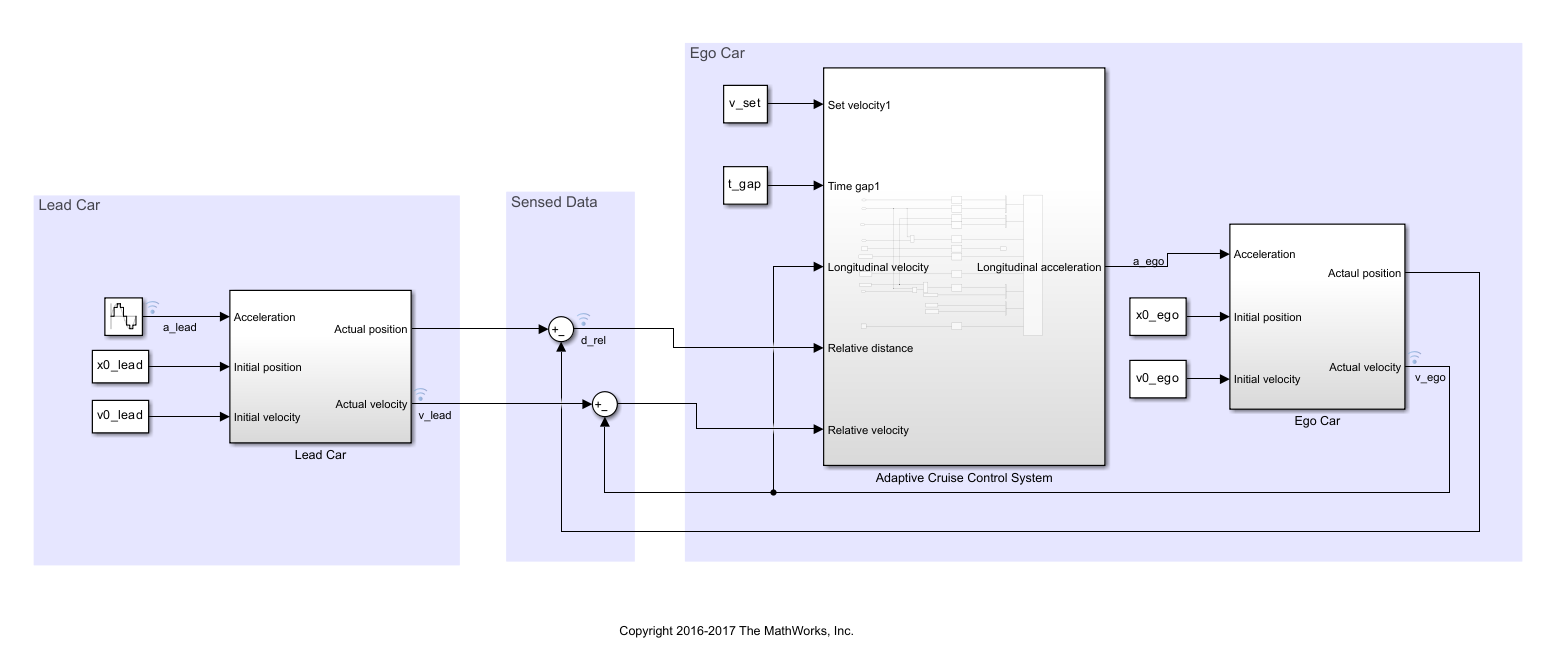
\includegraphics[width=0.8\textwidth]{figuras/simulink_model_for_lead_car_and_ego_car.png}
    \fonte{ O Autor adaptado de \cite{matwork-adaptive-cruise-control-using-model-predictive-controller}.}
\end{figure}

O sinal ( a\_{\text{des}}(t) ), produzido pelo bloco \textit{Adaptive Cruise Control System}, é empregado como entrada para um bloco \textit{MATLAB Function} que simula a resposta da pressão hidráulica do sistema de freio. Este bloco implementa a modelagem não linear da válvula hidráulica, conforme discutido anteriormente, e gera os sinais PWM correspondentes para a bomba e válvulas HSV/USV.

O código a seguir exemplifica a integração entre o controle preditivo e o subsistema hidráulico:

Essa integração possibilita analisar a coerência entre o controle de alto nível (ACC/MPC) e a atuação física do sistema de freio, demonstrando a viabilidade da arquitetura embarcada proposta. Os sinais de saída — pressão hidráulica, PWM da bomba e válvulas — são utilizados nas etapas seguintes para análise de desempenho e comparação com outras estratégias de controle. A Figura~\ref{fig:sinal_saida_bloco_controle_hidraulico_com_saida_modelo_acc_mcp} apresenta o comportamento do sistema sob diferentes condições de operação.

\begin{figure}[htbp]
    \centering
    %\caption{Sinal Saída Bloco Controle Hidráulico com Saída Modelo ACC MPC.}%
    \label{fig:sinal_saida_bloco_controle_hidraulico_com_saida_modelo_acc_mcp}
    \includegraphics[width=0.8\textwidth]{figuras/sinal_saida_bloco_controle_hidraulico_com_saida_modelo_acc_mcp.png}
    \fonte{ O Autor adaptado de \cite{Matlab2024}.}
\end{figure}


Apesar do modelo MPC permitir a consideração explícita de restrições e antecipação de comportamentos futuros, sua implementação embarcada demanda recursos computacionais significativos. Neste estudo, o MPC é utilizado apenas como referência para geração de sinais de teste, não sendo implementado diretamente no hardware. Futuras investigações poderão explorar a viabilidade de embarcar o controle preditivo, bem como avaliar o desempenho do sistema sob incertezas paramétricas e restrições operacionais mais rigorosas.


%####################################################################
%####################################################################
%####################################################################
%####################################################################
\section{Projeto do Controlador LQR}
\label{sec:controle-4-2}
O controle da pressão hidráulica no sistema de freio veicular embarcado demanda precisão, estabilidade e resposta adequada. Neste contexto, o Regulador Linear Quadrático (LQR) foi adotado como estratégia de controle digital, considerando sua capacidade de fornecer soluções ótimas para sistemas lineares e sua viabilidade computacional em aplicações embarcadas.

A literatura apresenta diversas alternativas para o controle de sistemas hidráulicos automotivos, incluindo abordagens baseadas em lógica difusa \cite{Pananurak2009}, controladores Proporcional-Integral (PI) \cite{YangYing2017}, Proporcional-Integral-Derivativo (PID) \cite{LuuAndLupu2019} e controle preditivo baseado em modelo (MPC) \cite{Tian2024, LihuaLuo2016}. Embora o MPC permita lidar com restrições e múltiplas variáveis, sua implementação em unidades de controle embarcadas pode ser limitada por requisitos computacionais elevados, decorrentes da necessidade de resolver problemas de otimização em tempo real, especialmente em plataformas com recursos restritos.

O LQR, por sua vez, oferece um compromisso entre desempenho e simplicidade, permitindo o projeto sistemático a partir de modelos linearizados, como o do subsistema hidráulico apresentado anteriormente. Sua aplicação possibilita a obtenção de sinais de controle suaves e estáveis, características desejáveis para evitar desgaste prematuro dos componentes e desconforto ao usuário.

A equação original do modelo hidráulico é dada por:

\begin{equation} \dot{p}_w = \frac{k_w}{A_w^2} C_d \cdot \alpha \cdot u \cdot \sqrt{\frac{2(p_m - p_w)}{\rho}} \end{equation}

A linearização em torno de um ponto de operação resulta nos coeficientes:

\begin{equation} a = \frac{\partial f}{\partial x} = -\frac{k_w}{A_w^2} C_d \alpha \sqrt{\frac{1}{2 \rho (p_m - p_w)}} \end{equation}

\begin{equation} b = \frac{\partial f}{\partial u} = \frac{k_w}{A_w^2} C_d \alpha \sqrt{\frac{2(p_m - p_w)}{\rho}} \end{equation}

Esses parâmetros são atualizados dinamicamente no bloco de controle, permitindo que o LQR se adapte às condições operacionais do sistema.

O controlador LQR busca minimizar a função de custo quadrática:

\begin{equation} J = \int_0^\infty (x^T Q x + u^T R u) dt \end{equation}

Os pesos ( Q ) e ( R ) podem ser ajustados segundo o erro de rastreamento e a pressão atual, promovendo maior robustez frente a variações de carga e dinâmica. Estratégias de ajuste automático desses pesos, ou mesmo a combinação com técnicas de controle robusto, podem ser consideradas em trabalhos futuros para lidar com incertezas mais pronunciadas.

O código a seguir exemplifica a implementação do controle LQR adaptativo para pressão hidráulica:

A Tabela~\ref{tab:parametros_lqr} apresenta os parâmetros físicos utilizados na simulação do controlador LQR:

\begin{table}[h!] 
\Caption{
\label{tab:parametros_lqr} Parâmetros físicos do subsistema hidráulico utilizados no controle LQR} 
\UNIFORtab{}{ 
    \begin{tabular}{ l | l | l | l } 
        \hline Parâmetro & Símbolo & Valor Típico & Unidade \\ 
        \hline Pressão da bomba (entrada) & $p_m$ & $10 \times 10^6$ & Pa \\ 
        \hline Densidade do fluido hidráulico & $\rho$ & 850 & kg/m³ \\ 
        \hline Área do cilindro da roda & $A_w$ & 0{,}002 & m² \\ 
        \hline Rigidez do cilindro da roda & $k_w$ & 20000 & N/m \\ 
        \hline Coeficiente de descarga da válvula & $C_d$ & 0{,}7 & — \\ 
        \hline Ganho PWM-área da válvula & $\alpha$ & $1 \times 10^{-6}$ & m² \\ 
        \hline 
    \end{tabular} }{ \Fonte{Elaborado pelo autor} } 
\end{table}

A aplicação do LQR ao subsistema hidráulico do sistema de freio veicular embarcado demonstrou-se adequada para os objetivos deste estudo, equilibrando desempenho, simplicidade de implementação e compatibilidade com sistemas embarcados. Futuras investigações podem explorar a integração com técnicas de controle robusto, modo deslizante (SMC) ou ajuste automático de parâmetros para ampliar a resiliência do sistema frente a incertezas e variações operacionais.

A Figura~\ref{fig:lqr_pressao_adaptativo_valvulas} demostra a aplicação do LQR ao subsistema hidráulico do sistema de freio veicular embarcado que se mostrou uma escolha adequada, equilibrando desempenho ótimo, simplicidade de implementação e compatibilidade com sistemas embarcados.

\begin{figure}[htbp]
    \centering
    \caption{Sinal Saída Bloco Controle Hidráulico com Saída Modelo ACC MPC.}
    \label{fig:lqr_pressao_adaptativo_valvulas}
    \includegraphics[width=0.8\textwidth]{figuras/lqr_pressao_adaptativo_valvulas.png}
    \fonte{ O Autor adaptado de \cite{Matlab2024}. }
\end{figure}

%Inclusive, a análise da literatura reforça essa decisão, destacando o LQR como uma alternativa eficiente frente a controladores clássicos e preditivos em contextos de controle digital da pressão indireta%.

%####################################################################
%####################################################################
%####################################################################
%####################################################################
%\section{Projeto do Observador de \textit{Luenberger}}%
\label{sec:controle-4-3}
Em sistemas embarcados de controle, nem sempre é possível medir diretamente todas as variáveis de estado relevantes para o desempenho do sistema. No contexto do controle da pressão hidráulica em sistemas de freio automotivo, sensores de pressão podem apresentar limitações, como ruído, atrasos ou até mesmo falhas intermitentes. Diante dessas restrições, a estimação de estados internos a partir de medições disponíveis torna-se uma estratégia fundamental para aumentar a confiabilidade e robustez do controle.

O Observador de \textit{Luenberger} é uma abordagem clássica e amplamente utilizada para estimar variáveis de estado em sistemas lineares, especialmente quando se dispõe de um modelo matemático razoavelmente preciso. Considerando o modelo linearizado do subsistema hidráulico, o observador pode ser descrito pelas seguintes equações:

\begin{equation}
\dot{x} = a x + b u, \quad y = c x
\end{equation}

Onde:
\begin{itemize}
 \item \( x = p_w \): pressão no cilindro da roda (estado do sistema)
 \item \( u \): sinal PWM aplicado à válvula
 \item \( y \): pressão medida (com ruído)
 \item \( a, b \): coeficientes do modelo linearizado
 \item \( c = 1 \): saída diretamente proporcional ao estado
\end{itemize}

O observador de \textit{Luenberger} é implementado como:

\begin{equation}
\dot{\hat{x}} = a \hat{x} + b u + L(y - \hat{y}), \quad \hat{y} = c \hat{x}
\end{equation}

O termo ( $L(y - \hat{y})$) representa a realimentação do erro de estimação, ajustando a dinâmica do observador para que a estimativa ( $\hat{x}$ ) possa convergir ao valor real de ( $x$ ). O ganho ( $L$ ) é escolhido de modo que o erro de estimação ( $e = x - \hat{x}$ ) seja capaz de evoluir de acordo com:

\begin{equation}
\dot{e} = (a - Lc)e
\end{equation}

A seleção adequada de ( $L$ ) é essencial para garantir a convergência e a estabilidade do observador, sendo comumente realizada por alocação de polos ou técnicas de otimização. Em aplicações práticas, a escolha do ganho pode ser influenciada por fatores como ruído de medição, incertezas paramétricas e requisitos de resposta dinâmica.

O exemplo a seguir, Código~\ref{cod:observador_luenberger},ilustra a implementação do observador de \textit{Luenberger} em MATLAB:



A simulação do observador deve evidenciar: 
\begin{itemize} 
    \item Convergência da estimativa ( $\hat{x}$ ) para o valor real de ( $x$ ) mesmo na presença de ruído. 
    \item Robustez frente a variações do sinal PWM e perturbações na medição. 
    \item Estabilidade da estimação ao longo do tempo. 
\end{itemize}

A Figura~\ref{fig:observador_pressao_luenberger} apresenta o desempenho do observador de \textit{Luenberger} na estimação da pressão hidráulica em tempo real.

\begin{figure}[htbp]
    \centering
    \caption{Sinal Saída Bloco Controle Hidráulico com Saída Modelo ACC MPC.}
    \label{fig:observador_pressao_luenberger}
    \includegraphics[width=0.8\textwidth]{figuras/observador_pressao_luenberger.png}
    \fonte{ O Autor adaptado de \cite{Matlab2024}. }
\end{figure}

Embora o Observador de \textit{Luenberger} seja uma solução eficiente para sistemas lineares, alternativas como o filtro de Kalman ou observadores robustos podem ser consideradas em cenários com maior incerteza, ou não linearidades acentuadas. A escolha da técnica de estimação deve levar em conta as características do sistema, a disponibilidade de sensores e os requisitos de desempenho da aplicação.

%####################################################################
%####################################################################
%####################################################################
%####################################################################
%\section{Validação Experimental e Integração Final}%
\label{sec:controle-4-4}

Após o desenvolvimento dos modelos matemáticos, do projeto do controlador LQR e da implementação do observador de \textit{Luenberger}, esta seção apresenta a simulação integrada do sistema embarcado de controle de freio com ACC. O objetivo é avaliar a integração dos blocos funcionais e examinar o desempenho do sistema no rastreamento da pressão hidráulica de referência, considerando aspecto de precisão e estabilidade.

A simulação contempla os seguintes blocos conectados sequencialmente:

\begin{itemize} 
    \item \textbf{ACC (Adaptive Cruise Control)}: responsável pela geração do sinal de aceleração desejada \(a_{\text{des}}\) a partir da distância e velocidade relativa ao veículo à frente. 
    \item \textbf{Conversor (\(a_{\text{des}} \rightarrow p_{w,\text{ref}}\))}: realiza a conversão da aceleração desejada em pressão hidráulica de referência, conforme a relação: 
          \[ p_{w,\text{ref}} = \frac{m \cdot a_{\text{des}}}{A_c} \] 
    \item \textbf{Controlador LQR Adaptativo}: determina o sinal PWM necessário para rastrear \(p_{w,\text{ref}}\), utilizando o modelo linearizado atualizado em tempo real. 
    \item \textbf{Observador de \textit{Luenberger}}: estima a pressão real \(\hat{p}_w\) a partir do sinal PWM e da pressão medida, contribuindo para a mitigação de ruídos e atrasos. 
    \item \textbf{Modelo Hidráulico}: simula a evolução da pressão real \(p_w\) em função do sinal PWM aplicado. 
\end{itemize}

A simulação integrada busca:

\begin{itemize} 
    \item Verificar a capacidade do sistema em rastrear a pressão hidráulica de referência derivada de \(a_{\text{des}}\). 
    \item Avaliar a suavidade e a estabilidade do sinal PWM gerado pelo controlador. 
    \item Analisar o erro de estimação entre \(p_w\) e \(\hat{p}_w\) ao longo do tempo. 
\end{itemize}

O Código~\ref{cod:controle_integrado} a seguir representa o núcleo da simulação embarcada, integrando o controlador LQR adaptativo e o observador de \textit{Luenberger}:

A simulação deve ser executada em um laço temporal (por exemplo, em um \textit{script Simulink} ou MATLAB), onde a cada passo de tempo:

\begin{enumerate}
 \item O modelo ACC fornece \(a_{\text{des}}\).
 \item Calcula-se \(p_{w,\text{ref}}\).
 \item O bloco \textbf{controle\_integrado} é chamado com os parâmetros do sistema.
 \item As saídas PWM, \(\hat{p}_w\) e \(\text{erro}_{\text{est}}\) são armazenadas para análise.
\end{enumerate}

A Figura~\ref{fig:controle_integrado_lqr_luenberger} apresenta a simulação integrada e permite validar o comportamento do sistema de controle embarcado em condições realistas. A arquitetura modular facilita a substituição de blocos por versões físicas (sensores reais, atuadores, etc.) em futuras etapas de implementação. Os resultados obtidos com essa simulação são fundamentais para comprovar a viabilidade do controle digital da pressão hidráulica em sistemas de freio com ACC.

\begin{figure}[htbp]
    \centering
    \caption{Sinal Saída Bloco Controle Hidráulico com Saída Modelo ACC MPC.}
    \label{fig:controle_integrado_lqr_luenberger}
    \includegraphics[width=0.8\textwidth]{figuras/controle_integrado_lqr_luenberger.png}
    \fonte{ O Autor adaptado de \cite{Matlab2024}. }
\end{figure}


%####################################################################
%####################################################################
%####################################################################
%####################################################################
\section{Análise de Robustez do Sistema de Controle}
\label{sec:controle-4-5}

Após o desenvolvimento dos modelos matemáticos, do projeto do controlador LQR e da implementação do observador de \textit{Luenberger}, esta seção apresenta a simulação integrada do sistema embarcado de controle de freio com ACC. O objetivo é avaliar a integração dos blocos funcionais e examinar o desempenho do sistema no rastreamento da pressão hidráulica de referência, considerando aspecto de precisão e estabilidade.

A simulação contempla os seguintes blocos conectados sequencialmente:

\begin{itemize} 
    \item \textbf{ACC (Adaptive Cruise Control)}: responsável pela geração do sinal de aceleração desejada \(a_{\text{des}}\) a partir da distância e velocidade relativa ao veículo à frente. 
    \item \textbf{Conversor (\(a_{\text{des}} \rightarrow p_{w,\text{ref}}\))}: realiza a conversão da aceleração desejada em pressão hidráulica de referência, conforme a relação: 
          \[ p_{w,\text{ref}} = \frac{m \cdot a_{\text{des}}}{A_c} \] 
    \item \textbf{Controlador LQR Adaptativo}: determina o sinal PWM necessário para rastrear \(p_{w,\text{ref}}\), utilizando o modelo linearizado atualizado em tempo real. 
    \item \textbf{Observador de \textit{Luenberger}}: estima a pressão real \(\hat{p}_w\) a partir do sinal PWM e da pressão medida, contribuindo para a mitigação de ruídos e atrasos. 
    \item \textbf{Modelo Hidráulico}: simula a evolução da pressão real \(p_w\) em função do sinal PWM aplicado. 
\end{itemize}

A simulação integrada busca:

\begin{itemize} 
    \item Verificar a capacidade do sistema em rastrear a pressão hidráulica de referência derivada de \(a_{\text{des}}\). 
    \item Avaliar a suavidade e a estabilidade do sinal PWM gerado pelo controlador. 
    \item Analisar o erro de estimação entre \(p_w\) e \(\hat{p}_w\) ao longo do tempo. 
\end{itemize}

O Código~\ref{cod:controle_integrado} a seguir representa o núcleo da simulação embarcada, integrando o controlador LQR adaptativo e o observador de \textit{Luenberger}:



A execução da simulação ocorre em um laço temporal, no qual, a cada iteração:

\begin{enumerate} 
\item O modelo ACC fornece \(a_{\text{des}}\). 
\item Calcula-se ($ p_{w,\text{ref}}$ ). 
\item O bloco \textbf{controle\_integrado} é chamado com os parâmetros do sistema. 
\item As saídas ( $PWM$ ), ( $\hat{p}w$ ) e ($ erro{est}$ ) são armazenadas para análise posterior. 
\end{enumerate}

A Figura~\ref{fig:controle_robusto_simulink} que apresenta os resultados da simulação integrada, permite avaliar o comportamento do sistema de controle embarcado em condições próximas às reais. A arquitetura modular adotada facilita a substituição de blocos por versões físicas (sensores e atuadores reais) em etapas futuras, bem como a integração com plataformas HIL para validação experimental mais abrangente.

\begin{figure}[htbp]
    \centering
    \caption{Sinal Saída Bloco Controle Hidráulico com Saída Modelo ACC MPC.}
    \label{fig:controle_robusto_simulink}
    \includegraphics[width=0.8\textwidth]{figuras/controle_robusto_simulink.png}
    \fonte{ O Autor adaptado de \cite{Matlab2024}. }
\end{figure}

Cabe ressaltar que, embora a simulação forneça evidências da viabilidade da abordagem proposta, limitações inerentes ao ambiente computacional e à modelagem adotada devem ser consideradas na interpretação dos resultados. Fatores como latência de sensores, ruído eletromagnético e tolerâncias de fabricação não são plenamente capturados nesta etapa. Futuras investigações poderão explorar a validação experimental em hardware real, bem como a análise de desempenho sob diferentes cenários operacionais e perturbações externas.


%####################################################################
%####################################################################
%####################################################################
%####################################################################
\section{Discussão Crítica} 
\label{cap:discussao_critica}

O desenvolvimento de um sistema de controle digital embarcado para o freio veicular com ACC representa um avanço relevante na interface entre teoria de controle, eletrônica embarcada e segurança automotiva. Contudo, como em todo projeto aplicado, é fundamental analisar criticamente as premissas, simplificações e limitações inerentes à abordagem adotada.

A modelagem do subsistema hidráulico, ainda que fundamentada em referências consolidadas, parte do pressuposto de linearidade em torno de pontos de operação e desconsidera efeitos não lineares mais complexos, como histerese das válvulas, variações térmicas do fluido, atrasos eletromecânicos e a evolução do coeficiente de atrito das lonas de freio.

Já estudos recentes sugerem que a consideração dinâmica desse coeficiente pode aprimorar a precisão da estimação da pressão de frenagem, especialmente em sistemas sujeitos a desgaste e variações operacionais \cite{ZhangWang2021}. Além disso, pesquisas sobre o projeto paramétrico de motores em sistemas de freio eletro-hidráulicos reforçam a importância de integrar modelagem precisa e validação experimental para garantir desempenho otimizado em aplicações reais \cite{MotorParametricDesign2023}. Essas simplificações foram necessárias para viabilizar a implementação em tempo real no microcontrolador automotivo, mas restringem a precisão do modelo em situações extremas ou sob condições operacionais variáveis.

A escolha do controlador LQR mostrou-se adequada do ponto de vista computacional e de desempenho para sistemas lineares. Sua capacidade de fornecer soluções ótimas com baixo esforço de controle e estabilidade é compatível com aplicações embarcadas. No entanto, o desempenho do LQR depende fortemente da qualidade da linearização e da seleção dos pesos $Q$ e $R$, que aqui foram ajustados de forma heurística.

 Em cenários com variações abruptas de carga ou parâmetros, pode haver degradação do desempenho, o que justifica a consideração de estratégias adaptativas ou robustas em projetos posteriores. Estratégias de controle coordenado de pressão, como as propostas em \cite{PressureCoordinatedControl2023}, têm se mostrado eficazes para lidar com essas variações e garantir maior robustez ao sistema de frenagem eletro-hidráulico.

A implementação do observador de \textit{Luenberger} contribuiu para a robustez do sistema, permitindo a estimação da pressão hidráulica mesmo na presença de ruído ou falhas de sensores. Entretanto, o observador pressupõe conhecimento preciso dos parâmetros do modelo, o que pode não se confirmar em ambiente real. A sensibilidade do ganho $L$ à localização dos polos do observador também requer atenção, pois ajustes inadequados podem comprometer a estabilidade da estimação. Alternativas como o filtro de Kalman ou observadores robustos podem ser exploradas para lidar com incertezas paramétricas e ruídos não gaussianos.

Outro aspecto relevante é a ausência de validação em hardware real. Embora as simulações em MATLAB/Simulink tenham demonstrado a coerência do modelo e a viabilidade do controle, a transição para um ambiente físico envolve desafios adicionais, como latência de sensores, ruído eletromagnético, tolerâncias de fabricação e falhas intermitentes. A integração com sensores reais, como radar e câmera do sistema ADAS, também não foi abordada nesta etapa, embora seja fundamental para a operação completa do ACC.

A arquitetura modular proposta, com separação clara entre controle de alto nível ACC e controle de baixo nível (pressão hidráulica), mostrou-se alinhada com práticas contemporâneas de engenharia de sistemas embarcados. Essa modularidade facilita a substituição de blocos por versões mais sofisticadas, como controladores preditivos MPC, técnicas de controle robusto ou observadores não lineares, sem comprometer a estrutura do sistema. Além disso, a adoção de plataformas HIL pode ser considerada para validação experimental mais abrangente, aproximando ainda mais o estudo das condições reais de operação.





\begin{comment}
\textbf{\textit{Everton sugere que como o trabalho sera feito em modelagem, que faca o detalhamento da modelagem mecânica do modelo de freio, capitulo estimativa de presa de frenagem e controle indireto. }}

    \subsection{Estimativa da Pressão de Frenagem}
\label{sec:controle-estimacao-pressao}

Embora o sistema conte com um sensor de pressão instalado no bloco hidráulico, a medição disponível reflete apenas a pressão na linha principal, não necessariamente a pressão efetiva na câmara de cada freio. Além disso, a presença de ruído, atraso de amostragem e quantização exige que o controlador utilize não apenas o valor medido, mas também uma estimativa dinâmica da pressão.

A dinâmica da pressão no freio pode ser descrita em função das vazões de entrada e saída, controladas pelas válvulas solenoides, e da atuação da bomba eletro-hidráulica. Dessa forma, a pressão instantânea pode ser aproximada por modelos baseados em balanço de massa e compressibilidade do fluido. Este modelo permite inferir a pressão na câmara do freio mesmo em intervalos em que a válvula está comutada ou quando o sensor apresenta comportamento ruidoso.

Assim, o sistema de controle utiliza uma combinação entre a pressão medida e a pressão estimada pelo modelo hidráulico. Essa estimativa é especialmente importante em situações de variações rápidas da demanda de frenagem, comuns em aplicações de ACC, nas quais a bomba precisa modular a pressão de forma contínua. A fusão entre o sinal medido e a estimativa permite reduzir o impacto de ruído e melhorar a estabilidade do controlador.


###########################################################################
##############################################################################
##############################################################################3
##########################################################################3

Perfeito, Elton — vamos **pegar o capítulo do jeito que está** e **organizar** para chegar exatamente onde você quer **sem sair gerando texto agora**. Vou te entregar:

1.  **Mapa de corte/manutenção** (o que fica e o que sai, já na ordem final)
2.  **Arquitetura do capítulo “Controle” reorganizada** (só títulos + 1–2 frases guia por item)
3.  **Esqueleto LaTeX pronto para colar** (com seções, labels e *placeholders*), incluindo **onde inserir a sua planta** (equações do `Bloco_Hidraulico`) e **onde usar o MPC como gerador de referência**
4.  **Checklist de pendências mínimas** (para cada bloco, o que precisa existir para a banca “enxergar” coerência)
5.  **Onde mover o que for secundário** (Apêndice)

***

## 1) O que manter, o que retirar (corte cirúrgico)

**Manter (com pequenos ajustes de ligação):**

*   **Introdução** do capítulo (primeiros parágrafos do ACC e escopo).
*   **Seção “Modelagem da Planta”** — mas **agora ela vai, de fato, apresentar a planta** (seu modelo `Bloco_Hidraulico`).
*   **Seção “Simulação com Controle Preditivo (MPC)”** — como **gerador de $$a_{\text{des}}(t)$$**, não como controlador embarcado.

**Retirar por ora (ou mover para apêndice/futuros trabalhos):**

*   LQR, Observador de Luenberger, Análise de Robustez, Tabelas/Figuras relativas a esses blocos e qualquer “placeholder de código” não preenchido.
*   “Tabela de Distâncias ACC” (se quiser manter, **mover para Introdução/Estado da Arte** ou usar **apenas como saturação do $$a_{\text{des}}$$** com 1 linha explicativa).

***

## 2) Arquitetura do capítulo “Controle” (versão enxuta e coerente)

> **Objetivo**: mostrar **(i)** a planta hidráulica que você REALMENTE usa, **(ii)** como o ACC/MPC gera a **referência de aceleração**, **(iii)** como você **converte para referência de pressão** e **(iv)** como a planta responde.  
> (Sem entrar ainda em LQR/observador.)

**Cap. Controle – índice proposto**

1.  **Introdução** *(manter, só ajustar 1 frase de escopo)*  
    – “Este capítulo apresenta a **planta hidráulica modelada**, o **mapeamento $$a_{\text{des}}\to p_{\text{ref}}$$** e os **ensaios de simulação** com o ACC/MPC como gerador de sinais.”

2.  **Modelagem da Planta** *(agora com a planta de fato)*  
    2.1 **Hipóteses e arquitetura hidráulica** (duas linhas: fluido compressível, câmara equivalente, válvulas *inlet/outlet*, bomba, reservatório)  
    2.2 **Equações do subsistema hidráulico** *(do seu `Bloco_Hidraulico`)*  
    – Balanceamento de volumes/pressão (compressibilidade):
    $$
    \dot P=\frac{\beta}{V}\big(Q_b+Q_{\text{in}}-Q_{\text{out}}-K_{\text{leak}}\,P\big)
    $$
    – Bomba (função de $$\omega_p$$ e contrapressão): $$Q_b(\omega_p,P)$$  
    – Válvulas como orifícios:
    $$
    Q_{\text{in}}=C_{v,\text{in}}A_{\text{in,max}}u_{\text{in}}\sqrt{\tfrac{2\,\max(P_{\text{sup}}-P,0)}{\rho}},\quad
    Q_{\text{out}}=C_{v,\text{out}}A_{\text{out,max}}u_{\text{out}}\sqrt{\tfrac{2\,\max(P-P_{\text{ret}},0)}{\rho}}
    $$
    – Pressão a montante $$P_{\text{sup}}$$ (reservatório / mestre / manifold pressurizado pela bomba).  
    2.3 **Sinais de controle e saturações** (definir domínios: $$u_{\text{in}},u_{\text{out}}\in[0,1]$$, $$\omega_p\ge0$$).  
    2.4 **Parâmetros de simulação** *(tabela curta; rotular como “parâmetros de simulação”, não “típicos”)*  
    2.5 **Onde fica o código** *(indicar Apêndice com a listagem da função)*

3.  **Conversor $$a_{\text{des}} \rightarrow p_{\text{ref}}$$**  
    – Apresentar **a ponte**: usar sua forma simples **explicitando** que é aproximação de cilindro equivalente:
    $$
    p_{\text{ref}}=\kappa\,\frac{m\,|a_{\text{des}}|}{A_{\text{eq}}}
    $$
    com nota de que $$\kappa$$ é fator de calibração (pode incorporar distribuição por eixo, raio efetivo e atrito).  
    – **Limites/saturações** (p. ex. $$0\le p_{\text{ref}}\le p_{\max}$$).

4.  **Simulação com ACC/MPC como gerador de referência** *(manter sua seção, mas com foco)*  
    – Citar o modelo `mpcACCsystem` (MathWorks) **apenas como fonte de $$a_{\text{des}}(t)$$**.  
    – Diagrama simples: $$a_{\text{des}}(t)$$$$\rightarrow$$ conversor $$\rightarrow p_{\text{ref}}(t)$$$$\rightarrow$$ **planta hidráulica** $$\rightarrow P(t)$$.  
    – **Cenários de teste** (3 curtos):
    *   S1: degrau de $$a_{\text{des}}$$ (–0.5 m/s²)
    *   S2: rampa (–0→–1 m/s² em 2 s)
    *   S3: pulso (–1 m/s² por 0.5 s)  
        – **Métricas**: tempo de subida 10–90%, tempo de acomodação, *tracking error* $$|P-P_{\text{ref}}|$$ (mesmo que em malha “quase aberta”, dá para avaliar coerência do modelo).

5.  **Resultados e discussão curta (plant response)**  
    – 1–2 gráficos: $$P(t)$$ vs $$p_{\text{ref}}(t)$$ para S1–S3 (legendas com parâmetros).  
    – 1 parágrafo: “onde o modelo atende / onde satura” (p.ex., limitação por $$Q_b$$, $$A_{\text{in}}$$, etc.).  
    – **Limitações**: sem controle fechado ainda; controle será foco de trabalho futuro (ou capítulo subsequente).

6.  **Limitações e próximos passos**  
    – Enumerar o que entra depois: PI/LQR, observador/estimador, validação HIL; considerar histerese de válvulas, temperatura do fluido.

**Apêndice**

*   **Listagem da função `Bloco_Hidraulico`** (com `\lstlisting` ou verbatim), e um mini-*README* dos parâmetros.
*   Se quiser, **diagramas Simulink** (prints) em apêndice também.

***

## 3) Esqueleto LaTeX (pronto para colar e preencher aos poucos)

> **Obs.:** É um esqueleto enxuto para você ajustar localmente. Onde escrevi “(preencher)”, basta pôr 2–3 linhas.

```latex
% ======================
\chapter{Metodologia Específica: Controle Digital Para um Sistema de Freio ACC}
\label{cap:controle}

% --- 1. Introdução (MANTER, só ajustar 1 linha final de escopo)
% (seu texto atual)
% Acrescente ao final:
% Este capítulo apresenta a planta hidráulica modelada, o mapeamento a_des -> p_ref e os ensaios de simulação com ACC/MPC como gerador de sinais.

% --- 2. Modelagem da Planta
\section{Modelagem da Planta}
\label{sec:controle-planta}

\subsection{Hipóteses e Arquitetura}
\label{sec:planta-hipoteses}
% (preencher) Fluido compressível (módulo β), volume equivalente V, válvulas inlet/outlet como orifícios, bomba acionada por ω_p, reservatório a P_ret, ponto de suprimento P_sup.

\subsection{Equações do Subsistema Hidráulico}
\label{sec:planta-equacoes}

\noindent\textbf{Balanço de compressibilidade:}
\begin{equation}
\dot P = \frac{\beta}{V}\,\big(Q_b + Q_{\text{in}} - Q_{\text{out}} - K_{\text{leak}}\,P\big).
\end{equation}

\noindent\textbf{Bomba (fonte de vazão com perda):}
\begin{equation}
Q_b = K_b\,\omega_p - K_{lb}\,P,\qquad Q_b \ge 0.
\end{equation}

\noindent\textbf{Válvulas como orifícios equivalentes:}
\begin{align}
Q_{\text{in}} &= C_{v,\text{in}} A_{\text{in,max}} u_{\text{in}} \sqrt{\frac{2\,\max(P_{\text{sup}}-P,0)}{\rho}},\\
Q_{\text{out}}&= C_{v,\text{out}}A_{\text{out,max}} u_{\text{out}}\sqrt{\frac{2\,\max(P-P_{\text{ret}},0)}{\rho}}.
\end{align}

\noindent\textbf{Pressão a montante da inlet:}
% (preencher brevemente)
% P_sup = P_ret + K_sup * (ω_p / 2π), limitado por P_sup,max  (ou outras arquiteturas)

\subsection{Sinais de Controle e Saturações}
\label{sec:planta-controle}
% (preencher) u_in, u_out ∈ [0,1], ω_p ≥ 0; políticas simples: por ora, perfis prescritos nos ensaios.

\subsection{Parâmetros de Simulação}
\label{sec:planta-parametros}
% (preencher) tabela pequena (β, V, ρ, P_ret, K_b, K_lb, C_v,in/out, A_in/out,max, K_sup, P_sup,max).
% Rotular como "Parâmetros de simulação". Fonte: calibração do autor.

\subsection{Listagem do Modelo}
\label{sec:planta-listagem}
A implementação computacional do modelo hidráulico encontra-se no Apêndice~\ref{ap:bloco-hidraulico}, sob a função \texttt{Bloco\_Hidraulico}.

% --- 3. Conversor a_des -> p_ref
\section{Conversão de Aceleração para Referência de Pressão}
\label{sec:controle-conversor}

\noindent\textbf{Relação de referência (cilindro equivalente):}
\begin{equation}
p_{\text{ref}}(t) = \kappa\,\frac{m\,|a_{\text{des}}(t)|}{A_{\text{eq}}},\qquad 0 \le p_{\text{ref}} \le p_{\max}.
\end{equation}
% (preencher 2 linhas) Nota sobre κ (calibração) e A_eq (área equivalente / distribuição por eixo).

% --- 4. Simulação com ACC/MPC (manter sua seção, porém focada)
\section{Simulação com Controle Preditivo (MPC)}
\label{sec:controle-mpc}
% (seu texto) Ajustar para: MPC da MathWorks utilizado como gerador de a_des(t).
% Inserir 3 cenários (S1, S2, S3) e métricas (rise time, settling, erro |P - p_ref|).

% --- 5. Resultados
\section{Resultados e Discussão}
\label{sec:controle-resultados}
% (preencher) 1-2 figuras com P(t) vs p_ref(t) nos cenários S1..S3 com legendas contendo parâmetros.

% --- 6. Limitações e Próximos Passos
\section{Limitações e Próximos Passos}
\label{sec:controle-limites}
% (preencher) listar ausência de malha fechada real, histerese de válvulas, temperatura, estimador; próximos passos: PI/LQR, observador, HIL, etc.

% --- Apêndice com a função
\appendix
\section{Listagem do Modelo Hidráulico (\texttt{Bloco\_Hidraulico})}
\label{ap:bloco-hidraulico}
% \lstinputlisting[language=Matlab]{Bloco_Hidraulico.m}
% ou colar como verbatim, se preferir
```

> **Observação:** Se você já usa um arquivo `.m`, recomendo `\lstinputlisting` (pacote `listings`) para manter sempre sincronizado.

***

## 4) Checklist mínimo por bloco (para “passar na banca”)

*   **Modelagem da Planta**  
    ☐ Equações **explícitas** (as mesmas da função)  
    ☐ Tabela **pequena** de parâmetros (com a palavra “simulação”)  
    ☐ Vínculo claro de símbolos ↔ variáveis do código (e.g., $$K_b \leftrightarrow$$ `Kb`)  
    ☐ Referência ao **Apêndice** onde está a função

*   **Conversor $$a_{\text{des}}\to p_{\text{ref}}$$**  
    ☐ Equação **curta** com $$\kappa$$ (calibração)  
    ☐ **Saturações** (limites de pressão)

*   **Simulação com ACC/MPC**  
    ☐ Dizer que o MPC é **apenas gerador de sinais**  
    ☐ Definir **3 cenários** e **métricas**  
    ☐ Gráficos com **legendas informativas** (parâmetros)

*   **Resultados**  
    ☐ Pelo menos **2 figuras** $$P(t)$$ vs $$p_{\text{ref}}(t)$$  
    ☐ 1 parágrafo **curto** explicando comportamento e limitações

*   **Apêndice**  
    ☐ Listagem do `Bloco_Hidraulico`  
    ☐ (Opcional) Print do diagrama Simulink do pipeline

***

## 5) Onde colocar o que sobrou (sem apagar seu trabalho)

*   **LQR, Observador, Robustez** → criar **Seção “Trabalhos Futuros”** (ou manter títulos comentados e citar no fim como roadmap).
*   “Tabela de Distâncias ACC” → **Introdução/Estado da Arte** ou **nota de saturação** no conversor (1 linha).

***

### Quer que eu monte **a Tabela de Parâmetros** já no formato LaTeX (com os seus nomes de variáveis do código) e um **mini-mapa de símbolos** (código ↔ equação) para colar em \S\ref{sec:planta-parametros}?

Se disser “sim”, eu te devolvo **só esses dois blocos prontos**, sem gerar texto extra.

\end{comment}
\end{comment}